\chapter{栈和队列}
先说栈。在实际应用中有很多类似栈的数据调度方式。想象冬天你去澡堂洗澡。你脱衣服的顺序一定是从外到内，而穿衣服刚好相反。如图\ref{fig:洗澡穿脱衣服的例子}。
\begin{figure}[htbp]
    \centering
    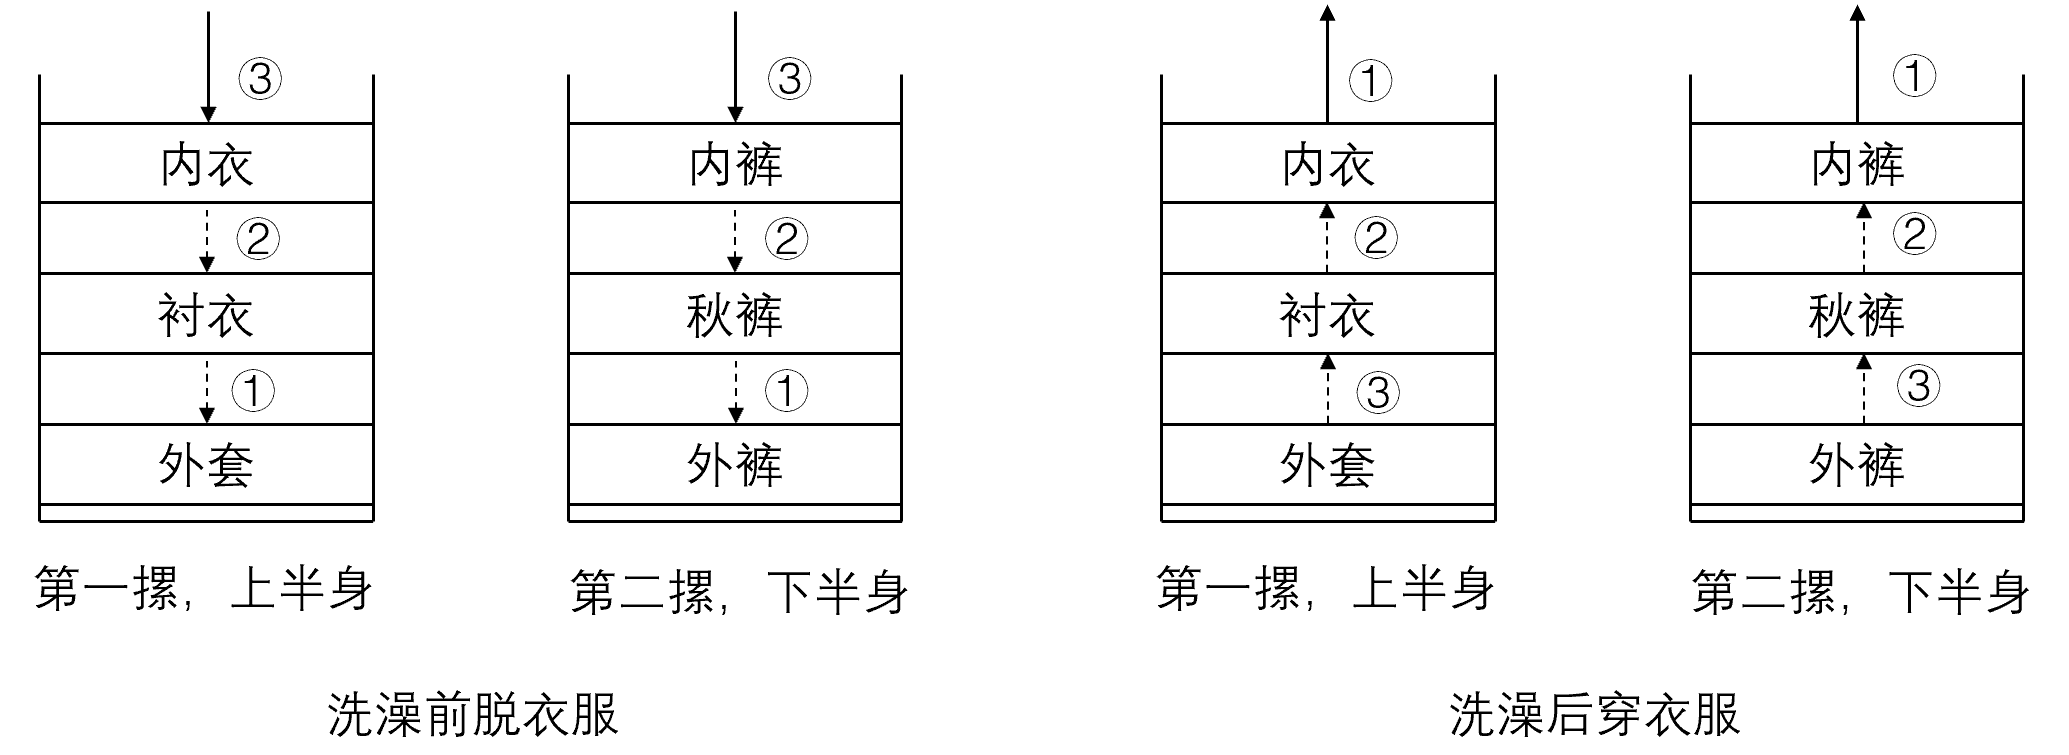
\includegraphics[width=0.78\textwidth]{assets/pics_and_ppts/ch3/洗澡穿脱衣服的例子.png}
    \caption{}
    \label{fig:洗澡穿脱衣服的例子}
\end{figure}

事实上，如果你将两摞衣物放在某个容器里，你会发现这个容器有这样的特点：先放入的在下方，后取出；后放入的在上方，先取出，称为\term{“后进先出”}，或者叫\term{“先进后出”}。
这样，其实你就是在将这两个容器当成两个\term{栈}来使用。\\


而\term{队列}就很好理解了，正得名于生活中的“队列”。想象某门店很火爆，门前排满了人，\uwave{队首}的人买完东西\uwave{出队}，新来的人\uwave{入队}到队尾。

接下来我们给出完整、严谨的\uwave{栈}和\uwave{队列}的定义。

\begin{definitionbox}
    \term{栈（Stack）}是只允许在一端进行插入或删除操作的\uwave{线性表}。
\end{definitionbox}
如图\ref{fig:栈的示意图}所示，允许插入或删除的那一端叫做\term{栈顶}，不允许插入或删除
的另一端叫做\term{栈底}，不包含任何元素的空表叫做\term{空栈}。栈的插入操作叫做\term{入栈}，删除操作叫做\term{出栈}，入栈和出栈通常也更生动地叫做“压栈”和“弹出”。
\begin{center}
    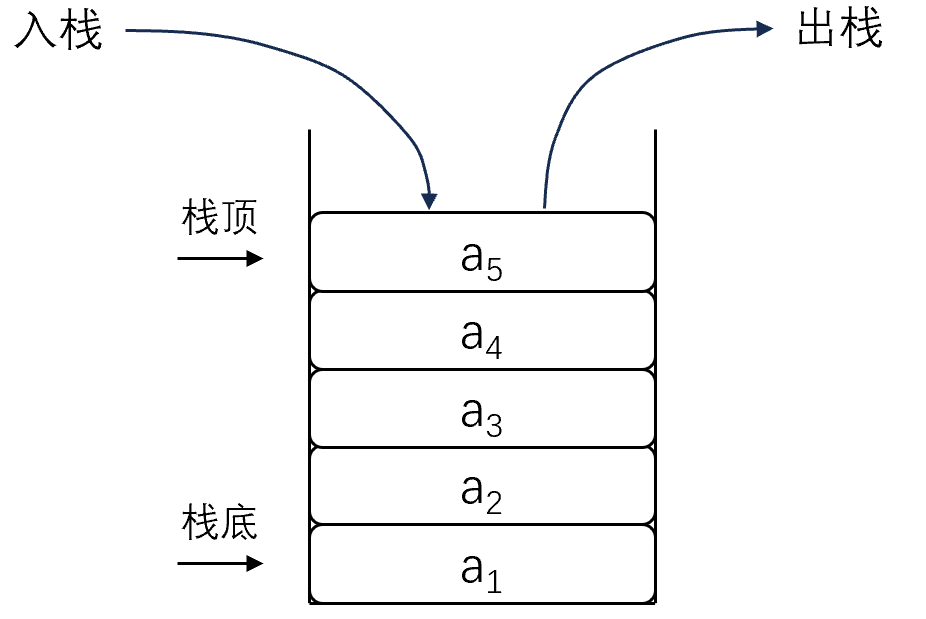
\includegraphics[width=0.48\textwidth]{assets/pics_and_ppts/ch3/栈的示意图.png}
    \captionof{figure}{栈的示意图}
    \label{fig:栈的示意图}
\end{center}

下面给出\term{队列}的定义。
\begin{definitionbox}
    \term{队列（Queue）}是只允许在其中一端插入、另一端删除的\uwave{线性表}。
\end{definitionbox}
如图\ref{fig:队列示意图}所示，允许出队的那一端叫做\term{队首}，允许入队的那一端叫做\term{队尾}，队列的插入操作叫做\term{入队}，删除操作叫做\term{出队}；
不包含任何元素的空表叫做\term{空队列}。
\begin{figure}[htbp]
    \centering
    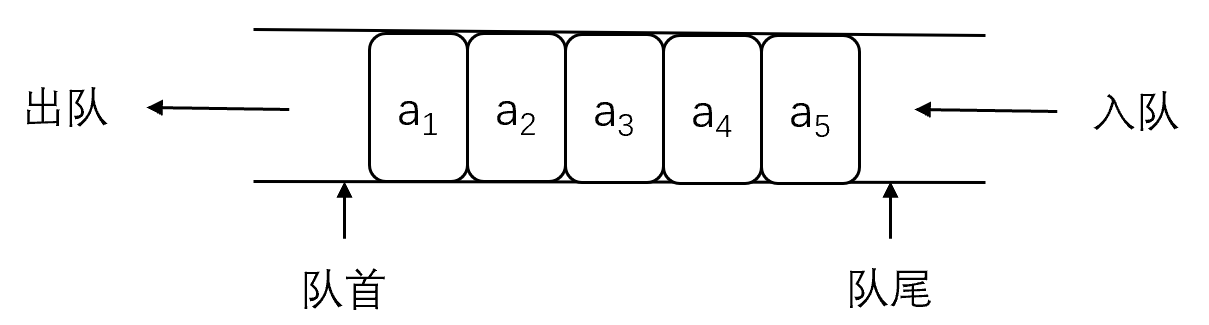
\includegraphics[width=0.55\textwidth]{assets/pics_and_ppts/ch3/队列示意图.png}
    \caption{队列示意图}
    \label{fig:队列示意图}
\end{figure}

很多人喜欢将栈和队列的特征进行对比，称\term{队列是先进先出（First In First Out, FIFO）的，栈是后进先出（Last In First Out，LIFO）的。}

以上便是栈和队列这两种逻辑结构的介绍，接下来我们研究如何实现栈和队列。
\section{栈}
上一章中我们研究了顺序表与链表的实现。既然栈是一种特殊的线性表，是不是可以用同样的物理存储来实现栈，并且对操作加以特殊限制呢？笔者建议大家在这里暂停，思考一下这个问题：
想象一下，分别用数组、链表该如何实现栈？如何设计是好的？会面临哪些问题吗？\\

此处应该有长时间留白......\\

开始。\\

相信大多数人的都会有明确而正确的思路：\\

1. 如果使用顺序表来实现栈，由于顺序表“尾插”、“尾删”均为O(1)的特性，可以将“表尾”作为“栈顶”，通过操作的定义和实现来限制该表
只能在表尾插入、删除，这样既有高效率，又满足栈的特点。如图\ref{fig:顺序栈实现示意图}所示，你可能会想到用一个int型变量top来动态维护“栈顶”的位置。
\begin{figure}[htbp]
    \centering
    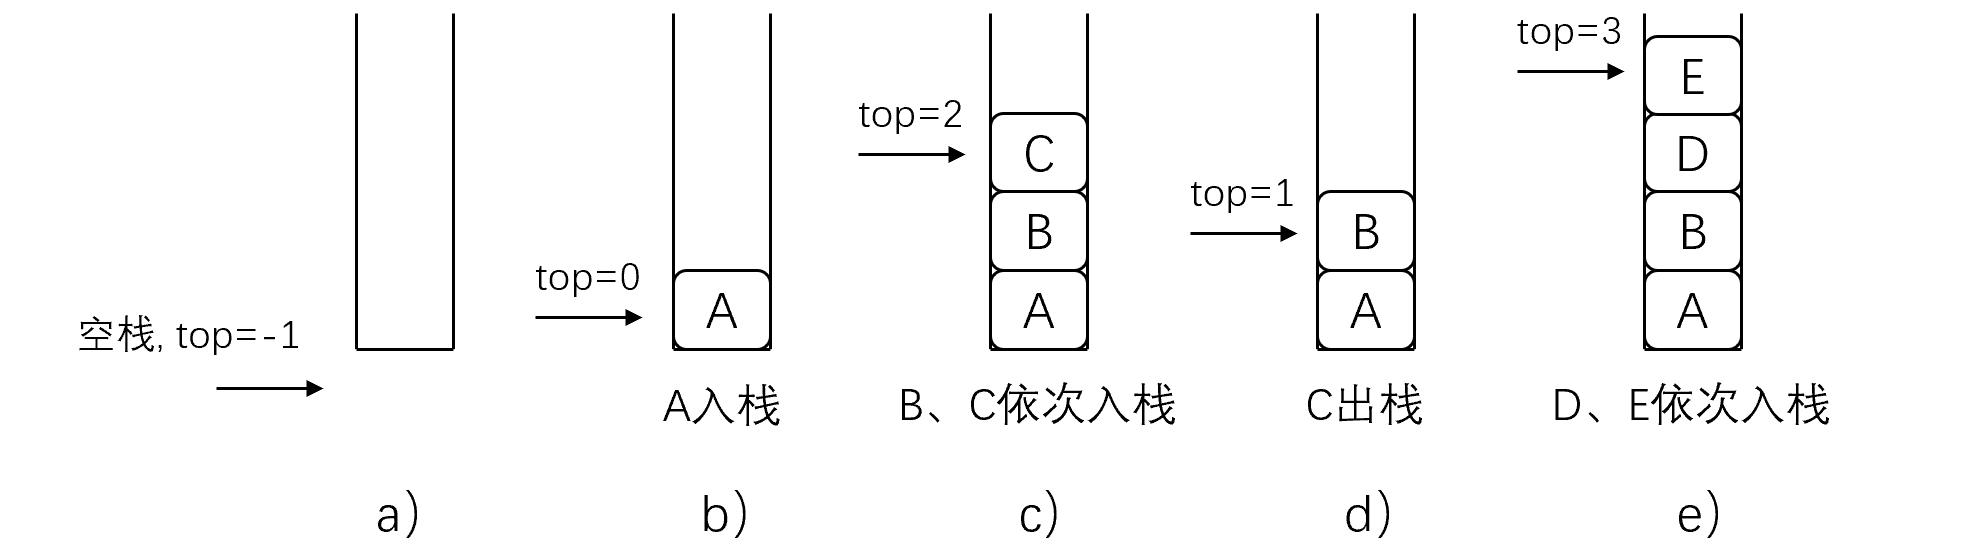
\includegraphics[width=0.78\textwidth]{assets/pics_and_ppts/ch3/顺序栈实现示意图.png}
    \caption{顺序栈实现示意图}
    \label{fig:顺序栈实现示意图}
\end{figure}

这个思路其实就是\term{顺序栈}的实现思路。采用顺序存储的栈称为\term{顺序栈}，它利用一组地址连续的存储单元存放自栈底到栈顶的数据元素，同时附设一个指针top，来
指示当前栈顶的位置。

顺序栈的存储结构如以下代码所示：
\begin{cppcode}
    #define MaxSize 100
    struct SeqStack {
        ElemType data[MaxSize]; // 存储实际的数据元素
        int top;    // 栈顶指针的下标
    };
\end{cppcode}
\begin{insightbox}
    你也许会发现，这特么不就是线性表么？你不就把current\_size换成top了么？没错，顺序栈和顺序表的关系确实有点暧昧不清。从存储结构角度看，二者存储结构完全相同，
    只不过语义不同：top表示栈顶元素的下标，空栈时为-1；而current\_size表示顺序表中元素的数量，空表时为0。二者之间微妙的关系在于，current\_size在数值上等于
    表尾元素（栈顶元素）的下标加一。而如果你将top的语义规定为“表尾元素（栈顶元素）的下一个位置”，那么就应将top初始化为0，而不是-1，此时top与current\_size
    语义虽然不同，但编码上是相同的。
\end{insightbox}



2. 如果使用链表来实现栈，由于链表“头插”、“头删”均为O(1)的特性，可以将“表头”作为“栈顶”，通过操作的定义和实现来限制该表
只能在表头插入、删除，这样同样既有高效率，又满足栈的特点。事实上，将链表的插入和删除操作限制在头部，即得到了\term{链栈}。

接下来我们分别给出顺序栈和链栈常见操作的实现。

\subsection{顺序栈的常见操作实现}
\minisection{1.顺序栈的初始化}
不难看出，初始化一个顺序栈仅需要将其栈顶指针top置为-1。
\begin{cppcode}
    int InitStack(SeqStack* S) {
        S.top = -1;
        return 1;
    }
\end{cppcode}
对于一个未初始化的顺序栈S:
\begin{cppcode}
    SeqStack S;
\end{cppcode}
就可以通过以下代码对S进行初始化：
\begin{cppcode}
    InitStack(S);
\end{cppcode}

\minisection{2.进栈操作}
top指针指向“当前栈顶元素”，因此进栈时要先移动指针到下一个“更高的”可用位置，再将元素放入该位置，此时指针仍指向栈顶。
\begin{cppcode}
    int Push(SeqStack& S, ElemType e) {    
        if(S.top == MaxSize - 1) {
            return 0;   // 栈已满，无法入栈
        }
        S.top += 1;
        S.data[S.top] = e;
        return 1;
    }
\end{cppcode}
如以下代码便可以为栈S压入一个值为3的元素：
\begin{cppcode}
    Push(S, 3);
\end{cppcode}

\begin{notebox}{初见提示}
    注意这里我们首次使用了C++的引用作为函数形参。"SeqStack\& S"中，符号"\&"并不是取地址的意思，而是表示形参S是一个SeqStack的\term{引用}类型。相信你也看出引用的作用了，
    类似使用指针一样，使用引用作为形参，同样可以改变函数栈外的原变量的值。关于引用的更多内容感兴趣的同学可以参考C++相关资料。
\end{notebox}

\minisection{3.出栈操作}
思想类似进栈，此处留白，请大家自行写出代码。
\begin{cppcode}
// 将栈S中当前的栈顶元素赋值给e，并将其弹出。
    int Pop(SeqStack& S, ElemType& e) {
        





    }
\end{cppcode}
\minisection{4.获取栈顶元素，但不出栈}
略。

\minisection{5.判断栈是否为空}
\begin{cppcode}
    int Empty(SeqStack S) {
        if(S.top == -1) return 1;   // Empty成立
        return 0;
    }
\end{cppcode}

\subsection{链栈的常见操作实现}
根据前面的介绍相信你已经看出来了，链栈的实现比链表还要简单：其他操作和链表几乎完全相同，而对于“插”和“删”，你只实现链表的“头插”和“头删”操作，而不实现任意位置的插入删除操作，你就得到了一个链栈。
显然链栈也可以采用带头结点和不带头结点的实现。这里拟采用带头结点的实现。

\begin{notebox}{提示}
    对于带头结点的实现，链表的第一个节点指针L指向头节点，L->next\_node指向的是第一个数据元素，即栈顶元素。
\end{notebox}

\minisection{1.链栈的入栈操作（实际上就是链表的“头插”操作）}
\begin{cppcode}
    int Push(ListNode* L, ElemType e) {
        ListNode* new_node = (ListNode*)malloc(sizeof(ListNode));
        new_node->data = e;
        new_node->next_node = L->next_node;
        L->next_node = new_node;
        return 1;
    }
\end{cppcode}

\minisection{2.链栈的出栈操作（实际上就是链表的“头删”操作）}
\begin{cppcode}
    int Pop(ListNode* L, ElemType& e) {
        if(L == NULL || L->next_node == NULL) {
            return -1;  
        }
        e = L->next_node->data;
        ListNode* node_to_free  = L->next_node;
        L->next_node = L->next_node->next_node;
        free(node_to_free );
        return 1;
    }
\end{cppcode}
显然实现一个栈没有必要使用双链表，更没有必要将首尾链接起来做成循环链表。

由于顺序栈和链栈就是有特殊限制的顺序表和链表，其优劣我们不再赘述，而是作为习题放在{\color{red}\textbf{习题2}}中。

\subsection{*浏览器的前进后退功能实现}
这里给出一个作为思维训练、理解栈的意义的极好的例子。大家应该都用过浏览器的“后退”和“前进”功能，如图\ref{fig:浏览器的前进后退示意}。当你按住鼠标右键从右向左滑动，
或者点击右键选择“后退”时，浏览器会访问你上一个访问过的网页，向右滑或点“前进”则回到上一个回退前的网页（如果你没用过，建议先打开浏览器试一下）。
\begin{figure}[htbp]
    \centering
    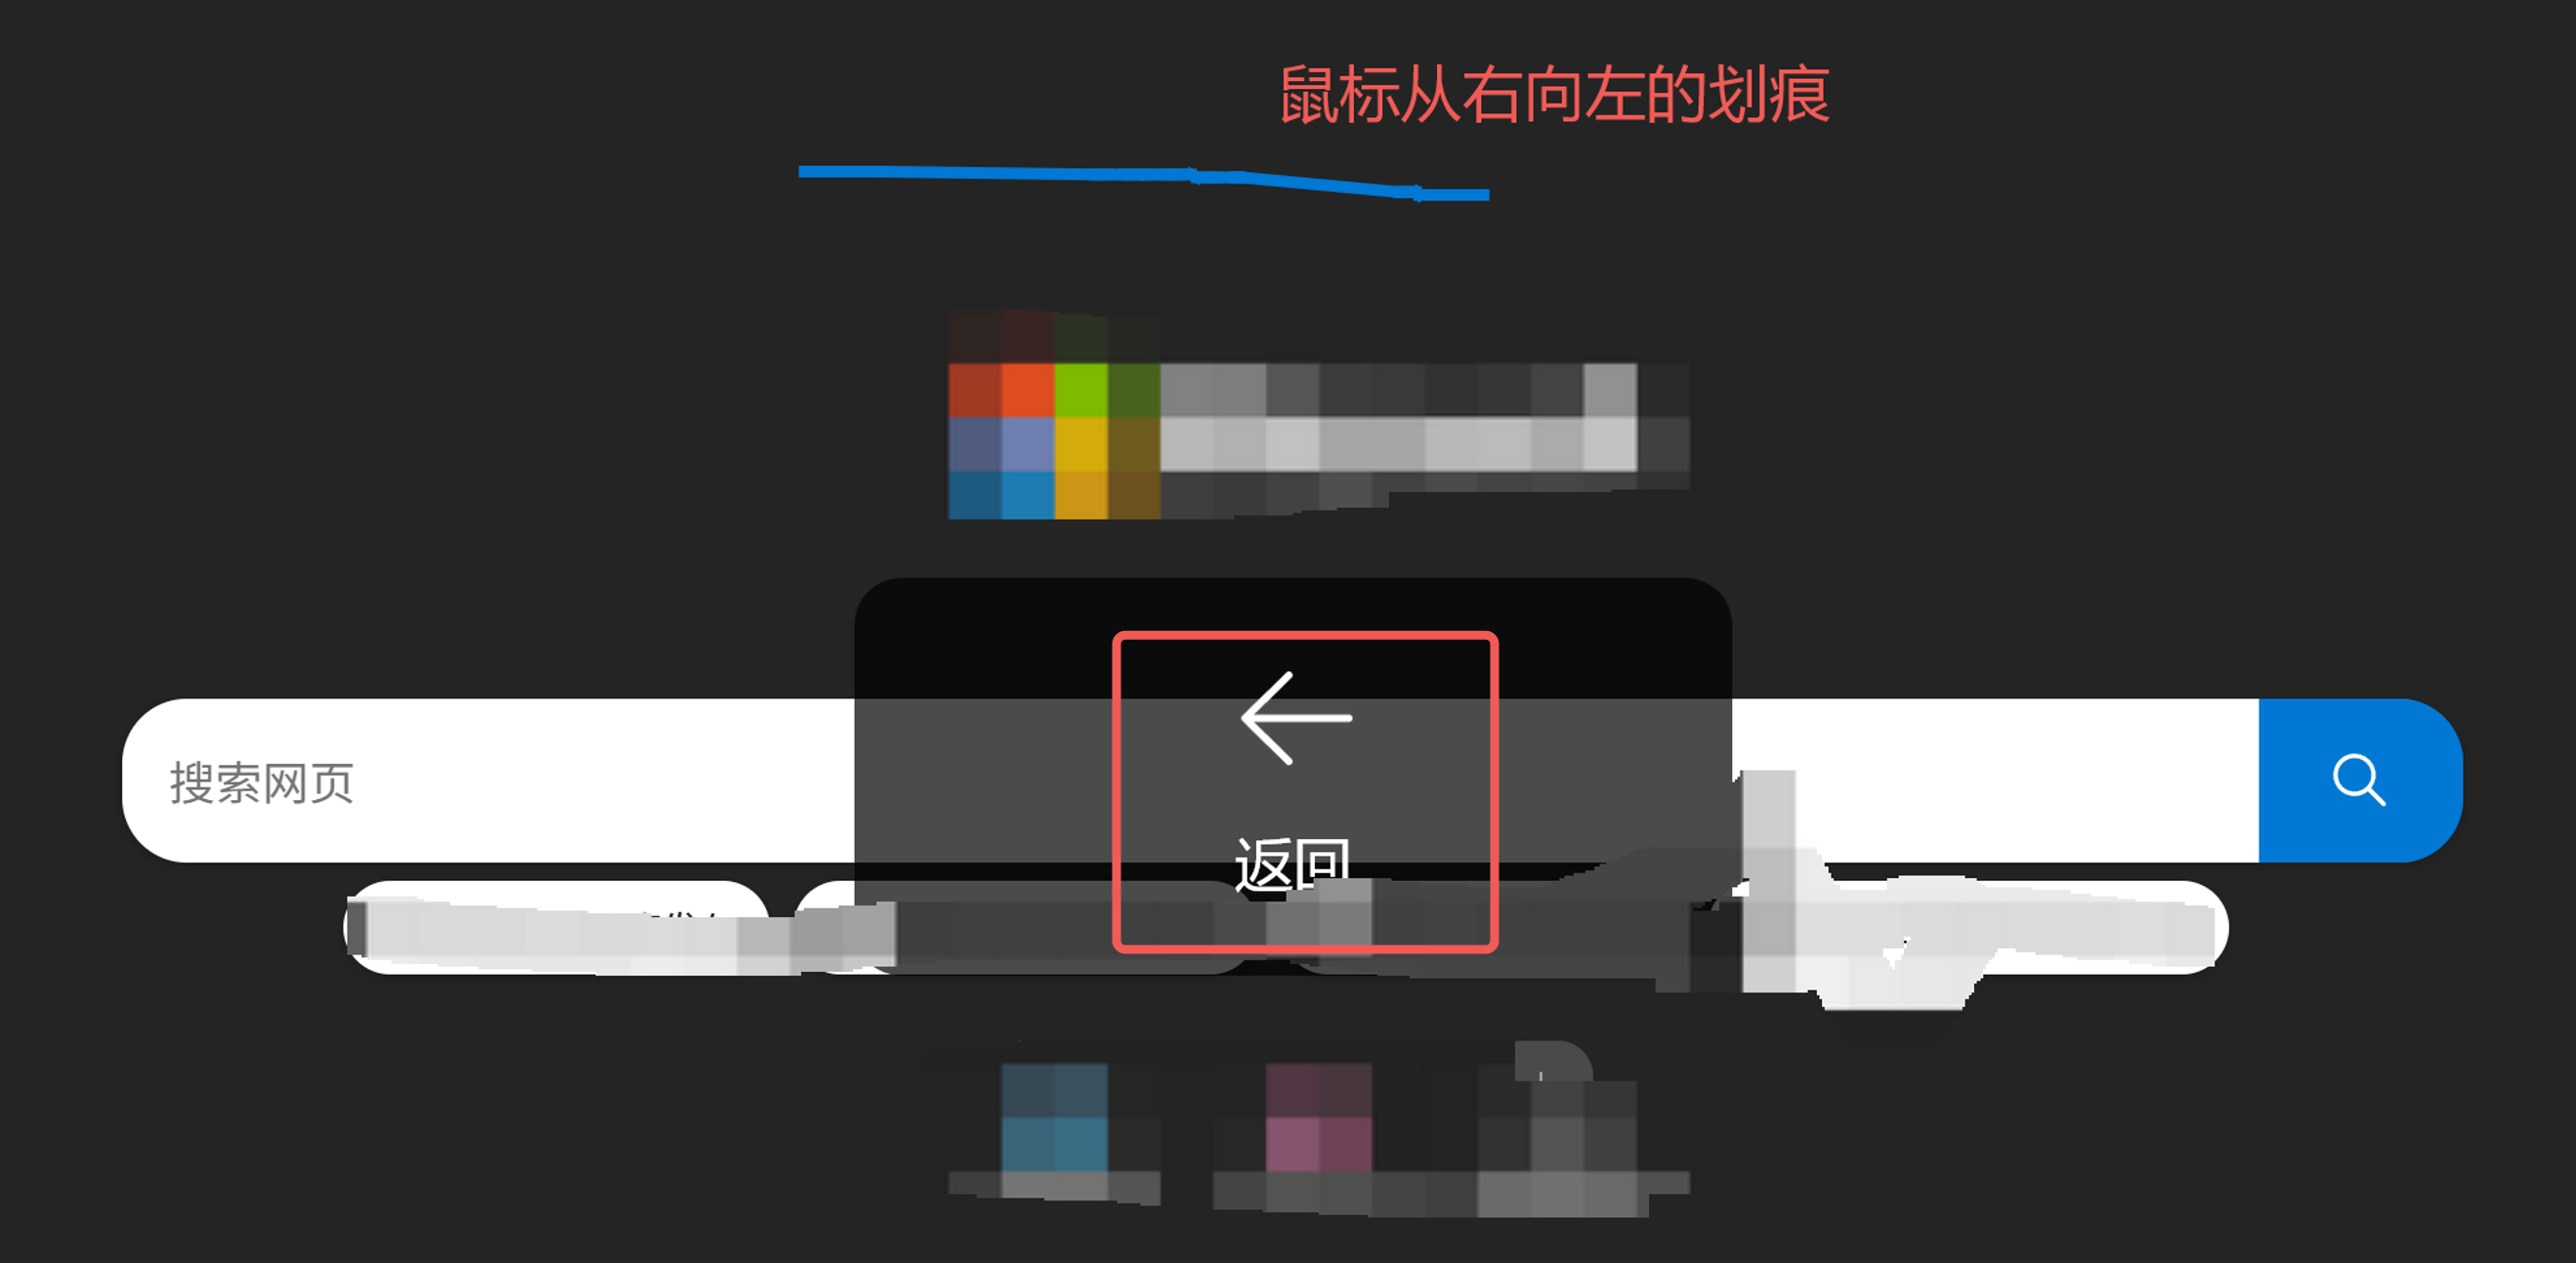
\includegraphics[width=0.6\textwidth]{assets/pics_and_ppts/ch3/浏览器的前进后退示意.png}
    \caption{}
    \label{fig:浏览器的前进后退示意}
\end{figure}
假设你已经访问过了：
\begin{bulk}
    网页1 -> 网页2 -> 网页3 
\end{bulk}
此时你处在网页3，点击“后退”，会回到网页2，再后退，回到网页1，再前进，回到网页2，再前进，回到网页3。

假设：\\
1.用户随时可能访问一个新的网站；\\
2.用户随时可能点击“后退”（鼠标左滑）；\\
3.用户随时可能点击“前进”（鼠标右滑）。\\
如果你是某浏览器的实现者，请你实现这个功能，要求当用户点击“前进”或“后退”时，能迅速地拿到对应网页的地址。

提示：网页地址（如https://xxxxxx）可以用一个char的数组（或string类型）来表示。你可以用任何你喜欢的方式来模拟用户的输入，并让你的程序做出合理反应。\\

此处应该有留白。\\

具体的模拟方式各有千秋，我们只给出核心算法的实现思路。不难看出，当用户访问了若干页面之后：
\begin{bulk}
    网页1 -> 网页2 -> 网页3
\end{bulk}
“后退”操作实际上就是依次访问与之前的顺序相反的页面，满足“后进先出”的特点，因此用户每访问一个\uline{新网页B}，我们就可以将用户所处在的\uline{当前网页A}
压入一个栈back\_stack，当用户进行后退时，取出栈顶网页访问即可。back\_stack语义上可以理解为：为用户的后退行为而预备的一个栈，栈顶元素永远是
用户此时点击后退时所要访问的页面。

还有前进操作。“后退”的顺序是与用户主动访问的新网页顺序相反，不难看出，“前进”的顺序是与“后退”相反的。因此可以维护令一个栈forward\_stack，用户未进行过后退操作时该
栈为空，当用户连续进行“后退”时，将网页依次压入栈forward\_stack。需要注意：当用户访问了一个新网页后无法“前进”，需要清空forward\_stack重新期待用户的下一次后退操作。
流程如图\ref{fig:使用两个栈实现浏览器前进后退}所清晰地展示。

\begin{figure}[htbp]
    \centering
    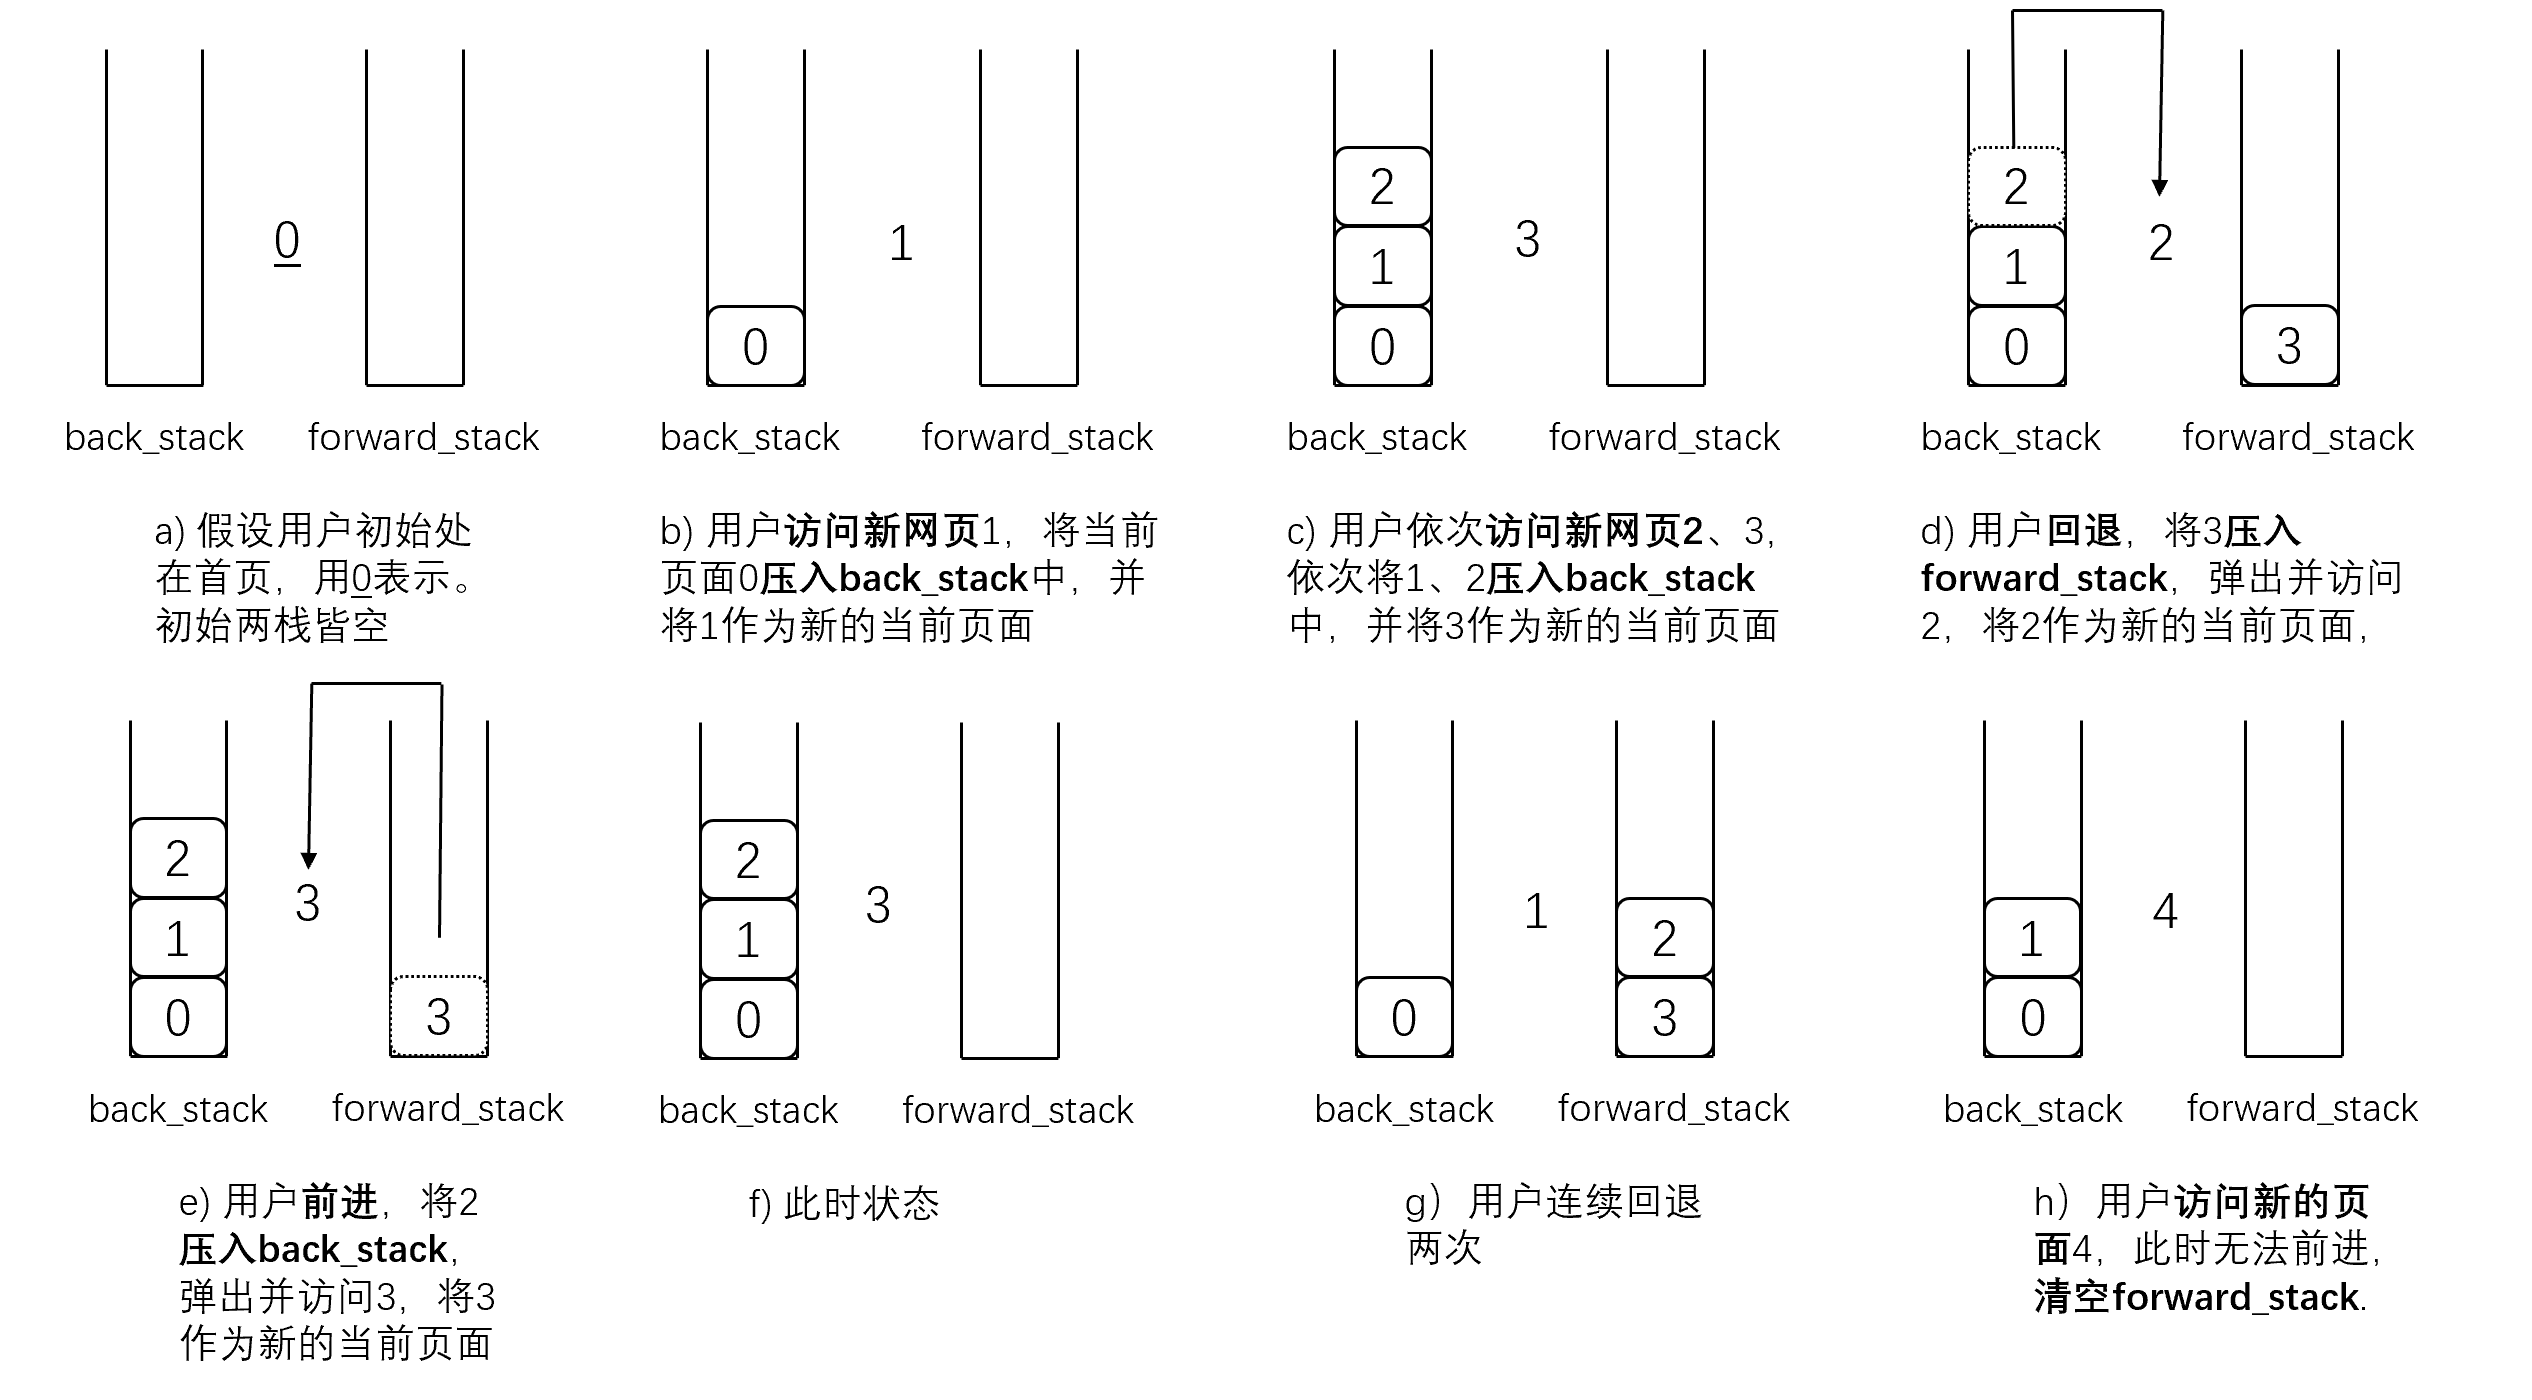
\includegraphics[width=1.15\textwidth]{assets/pics_and_ppts/ch3/使用两个栈实现浏览器前进后退.png}
    \caption{使用两个栈实现浏览器前进后退}
    \label{fig:使用两个栈实现浏览器前进后退}
\end{figure}

\subsection{*“函数栈”、“调用栈”是啥？}
相信大家从未注意但一个很有趣的事实是，函数调用、返回的顺序恰好具有“后进先出（LIFO）”的特点。如：
\begin{cppcode}
    void C() {
        return ;
    }
    void B() {
        C();
    }
    void A() {
        B();
    }
    int main() {
        A();
        return 0;
    }
\end{cppcode}
程序实际执行的顺序是：main -> A -> B -> C -> B -> A -> main -> 退出。函数执行结束时，需要返回上层，因此调用一个新函数时，需要将当前函数的上下文信息压入一个记录“函数调用
记录”的栈中（是不是有点像浏览器？）。从更底层的开发者角度来看，“调用栈”就是存放这些函数信息的一个栈，栈中的每一个元素是相应的函数上下文信息，如函数参数、局部变量
、返回地址等。

但对于应用程序员，特别是C/C++程序员来说，“调用栈”或“函数栈”通常存在其他角度的含义。对于C/C++来说，非静态局部变量存放在栈区，其可访问区域仅在函数内部。如：
\begin{cppcodeNum}[label={code:调用栈示例代码}]
    int f(int t) {
        int a = 10;
        t = t + a;
    }

    int main() {
        int x = 2;
        f(x);
        return 0;
    }
\end{cppcodeNum}
事实上，调用函数时，操作系统通常会为其分配一个栈区空间，其局部变量便存储在这个栈区空间中。main函数中以x为参数调用f(x)，仅仅是将x的值\uwave{拷贝}给了“栈区变量”t。
因此，这种场景下我们常称t是“f的函数栈（或调用栈）中的一个栈变量”，此时“函数栈”或“调用栈”的含义便是内存中的“栈区”空间。

\begin{notebox}{提示}
    事实上，函数的形参可以理解为函数栈中的一个局部变量。如代码\ref{code:调用栈示例代码}，以x为实参调用f，可以等效理解为如下伪代码：
    \begin{cppcode}
        int f() {
            int t;
            t = x;  // 外界传入的x的值拷贝给t
            ...

        }
    \end{cppcode}
    这也进一步解释了值传递无法改变函数栈外的原变量的值，而需要通过指针传递。
\end{notebox}

\section{队列}
如前所述，队列同样是一种特殊的线性表，因此队列同样可以有顺序存储和链式存储两种物理结构，并在顺序表或链表的基础上实现特殊机制。队列的链式存储稍简单些，
我们先研究链式存储，再研究顺序存储。

\subsection{队列的链式存储}
队列需要实现两个操作：在链表的头部删除元素、尾部插入元素。单链表头插本身可以达到O(1)。我们只要额外保存一个链表的尾指针，那么在尾部插入元素的操作也可以达到O(1)。显然
链式队列同样可以带头结点或不带头节点，这里拟采用带头节点的实现。

第二章中已经给出过链表节点的定义，这里为了体现出节点是队列的节点，我们把结构改个名字：
\begin{cppcode}
    struct QueueNode {
        ElemType data;
        struct QueueNode* next_node;
    };
\end{cppcode}
额外保存一个表尾指针来使出队操作时间达到O(1)：
\begin{cppcode}
    typedef struct {
        struct QueueNode* front;     // 表头(队首)指针，指向头节点
        struct QueueNode* rear;     // 表尾(队尾)指针，指向最后一个节点
    }LinkQueue;
\end{cppcode}
以上代码将LinkQueue定义为一个“链队列”类型。有了如上定义，我们就可以用如下代码定义链队列对象：
\begin{cppcode}
    LinkQueue happy_linkqueue;  // 定义一个开心的链队列
    LinkQueue sad_linkqueue;    // 定义一个悲伤的链队列
\end{cppcode}
一个链队列如图\ref{fig:带头结点的链式队列示意图}所示。前面的happy\_linkqueue以及sad\_linkqueue都是定义了但未初始化的。接下来我们给出链式队列的常见操作实现（带头结点）。
\begin{figure}[htbp]
    \centering
    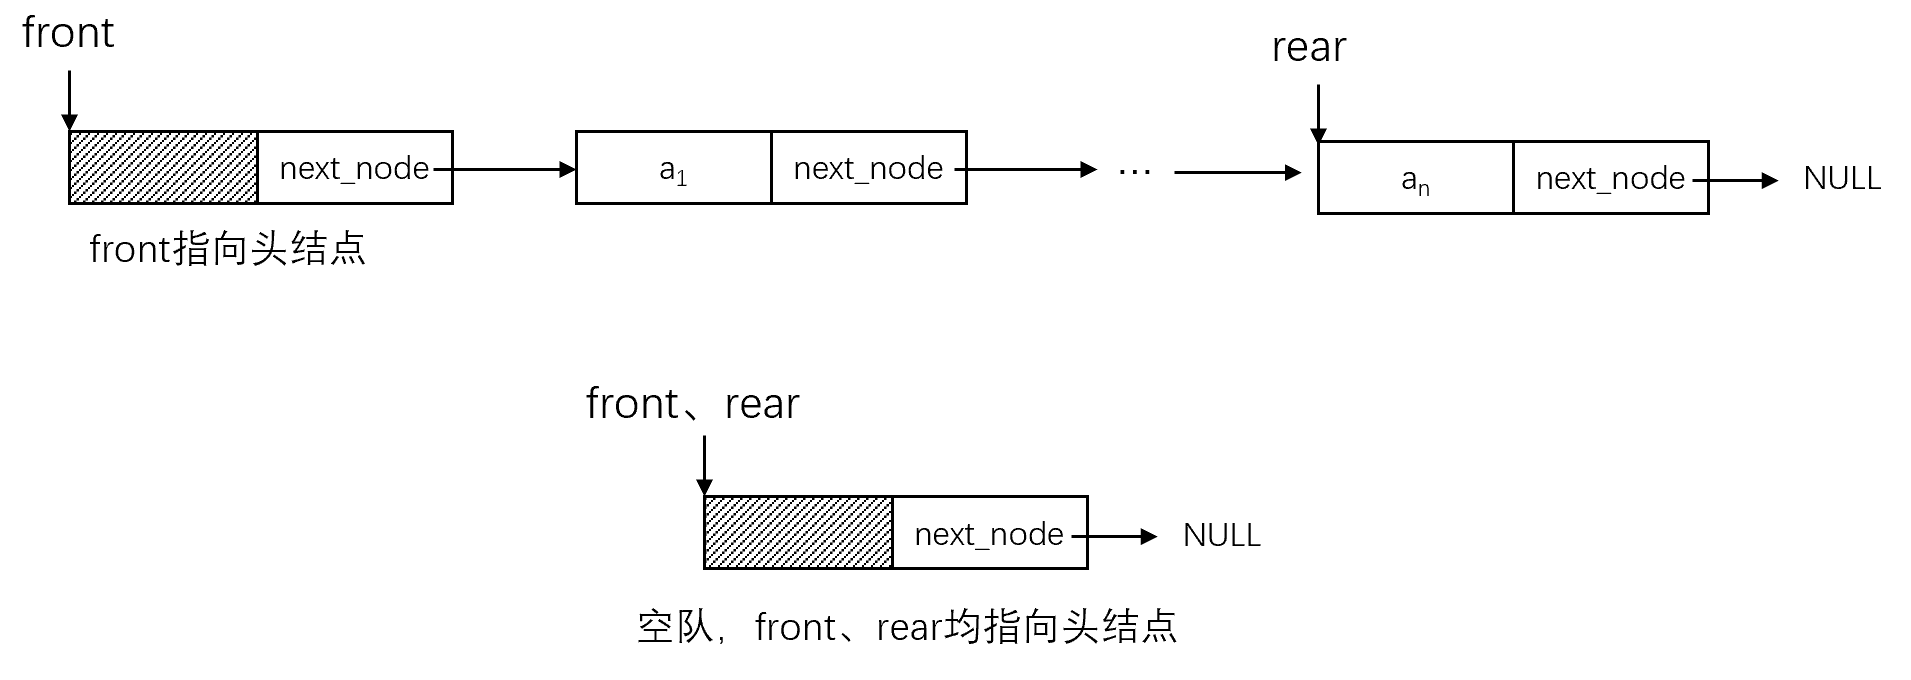
\includegraphics[width=0.85\textwidth]{assets/pics_and_ppts/ch3/带头结点的链式队列示意图.png}
    \caption{带头结点的链式队列示意图}
    \label{fig:带头结点的链式队列示意图}
\end{figure}

\minisection{1.初始化操作}
\begin{cppcode}
    int InitLinkQueue(LinkQueue& q) {
        q.front = (QueueNode*)malloc(sizeof(LinkQueue));     // 为头节点分配空间
        q.rear = q.front;    // 由于插入时要在尾后插入，所以rear初始指向头节点符合条件

        q.front->next_node = NULL;
        q.rear->next_node = NULL;
        return 1;
    }
\end{cppcode}
使用：
\begin{cppcode}
    InitLinkQueue(happy_linkqueue); // 初始化开心的链队列
    InitLinkQueue(sad_linkqueue);   // 初始化悲伤的链队列
\end{cppcode}

\minisection{2.判断是否空队}
\begin{cppcode}
    int Empty(LinkQueue q) {
        if(q.front == q.rear) {
            return 1;
        } 
        return 0;
    }
\end{cppcode}

\minisection{3.入队操作（尾插）}
\begin{cppcode}
    int EnQueue(LinkQueue& q, ElemType e) {
        if(q.front == NULL || q.rear == NULL) {
            return -1;  // 你给我个没初始化的队列我咋给你插入元素？
        }
        QueueNode* nwe_node = (QueueNode*)malloc(sizeof(QueueNode));
        nwe_node->data = e;
        // 操作链条
        nwe_node->next_node = NULL;
        q.rear->next_node = nwe_node;

        // 更新尾指针
        q.rear = nwe_node;
        return 1;
    }
\end{cppcode}

\minisection{4.出队操作（头删）}
一般情况下出队不会改变尾指针的指向，但需要注意一个特殊情况，即队列中仅有一个节点，如图\ref{fig:仅有一个数据节点的队列}所示。此时队首节点就是队尾节点，出队后，
队列变成空队，需要维护队尾节点指针，将其指向头节点。
\begin{cppcode}
    int DeQueue(LinkQueue& q, ElemType& e) {
        if(q.front == NULL || q.rear == NULL) {
            return -1;
        }
        if(q.front == q.rear) {
            return 0;   // 空队
        }   // 注意代码若能走出这个if，说明队中至少有一个数据节点，可以直接安全地访问q.front->next_node的data域或next_node域。
        e = q.front->next_node->data;
        QueueNode* t = q.front->next_node;
        q.front->next_node = q.front->next_node->next_node;

        // 若队列仅有一个节点，更新q.rear
        if(q.rear == t)
            q.rear = q.front;
        }
        free(t);
        return 1;
    }
\end{cppcode}
\begin{figure}[htbp]
    \centering
    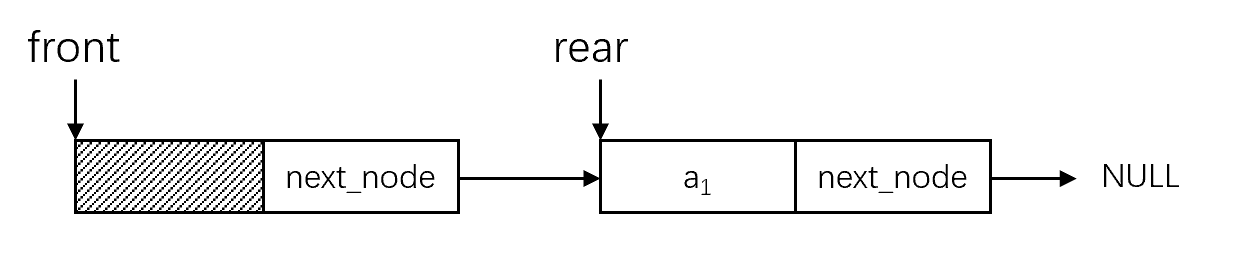
\includegraphics[width=0.70\textwidth]{assets/pics_and_ppts/ch3/仅有一个数据节点的队列.png}
    \caption{仅有一个数据节点的队列}
    \label{fig:仅有一个数据节点的队列}
\end{figure}

\subsection{队列的顺序存储}
不难想到，要在顺序存储的线性表上实现一个队列，最简单的做法就是标记两个指针（数组下标）front和rear，分别指向队头和队尾，初始时将front和rear均置为0即可，这样我们
可以规定front始终指向队首元素，rear始终指向队尾元素的下一个可插入位置。
\begin{cppcode}
    #define MaxSize 100
    struct SeqQueue {
        ElemType data[MaxSize];
        int front;  // 队头，初始时为0
        int rear;   // 队尾，初始时为0
    };
\end{cppcode}


如图\ref{fig:在顺序表上实现队列}，入队时将元素插入到队尾并推移队尾指针，出队时推移队头指针。
\begin{figure}[htbp]
    \centering
    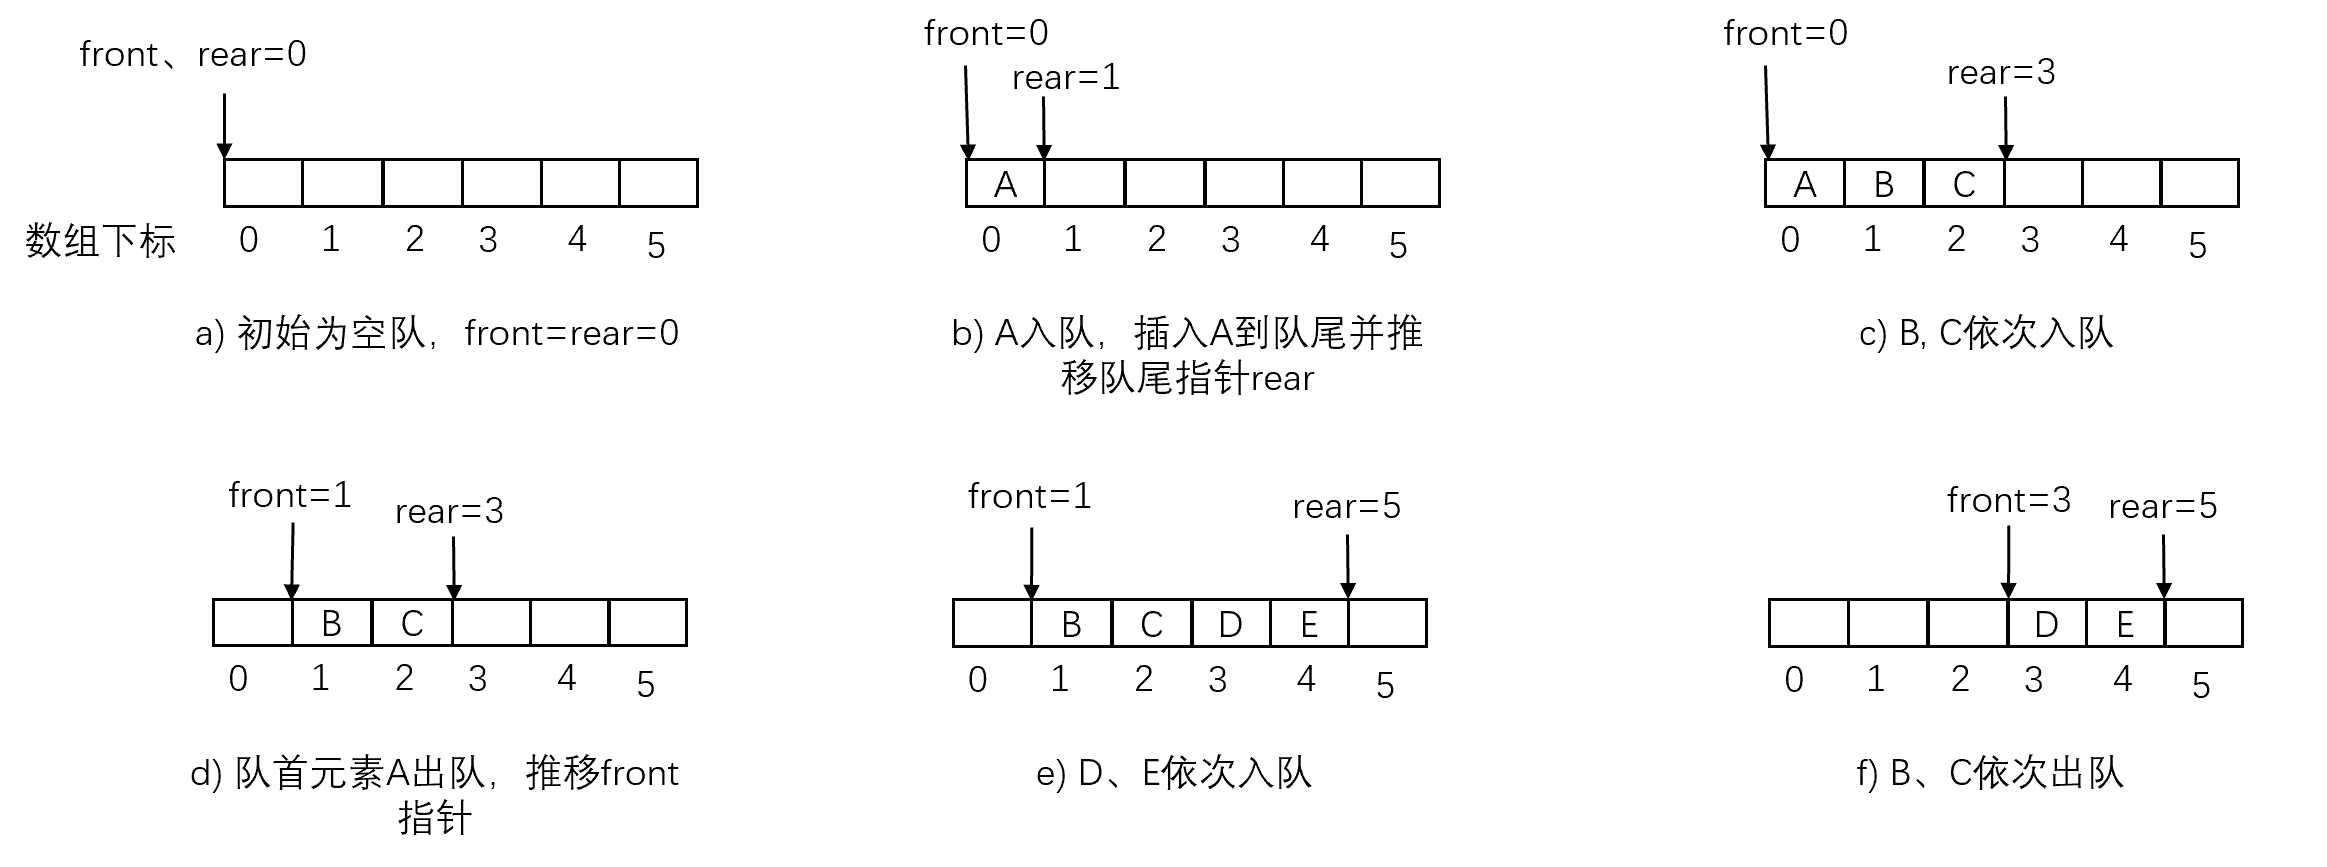
\includegraphics[width=1.05\textwidth]{assets/pics_and_ppts/ch3/在顺序表上实现队列.png}
    \caption{在顺序表上实现队列}
    \label{fig:在顺序表上实现队列}
\end{figure}

然而，一个看似简单的问题很快就会出现：

\begin{quote}
当rear已经走到了数组的尽头，而数组的前半部分却明明还有大量空闲空间时，我们还能继续入队吗？
\end{quote}

例如，一个容量为10的队列，经过几次入队、出队操作后，可能变成：

\[
\underbrace{\square\ \square\ \square\ \square}_{\text{已经出队，空闲}}
\quad
\underbrace{A\ B\ C\ D\ E\ F}_{\text{队列中的元素}}
\]

此时数组中明明还有4个空闲位置，但如果我们把数组看成一条只能从左向右移动的“道路”，rear已经走到了道路的尽头。按照普通顺序表的存储方式，我们似乎只能无奈地宣布：

\[
\text{“队列满了。”}
\]

可是，真的满了吗？

显然不是。相信聪明的你已经想到了，如图\ref{fig:循环队列示意图}所示，当rear走到尽头时，我们可以让rear“回到起点”，继续利用那些已经空闲了的空间，
\term{让rear始终“追着front跑”，当rear真正追上front时，确实没有可利用的空间了，此时才是真正的“队满了”}。
\begin{figure}[htbp]
    \centering
    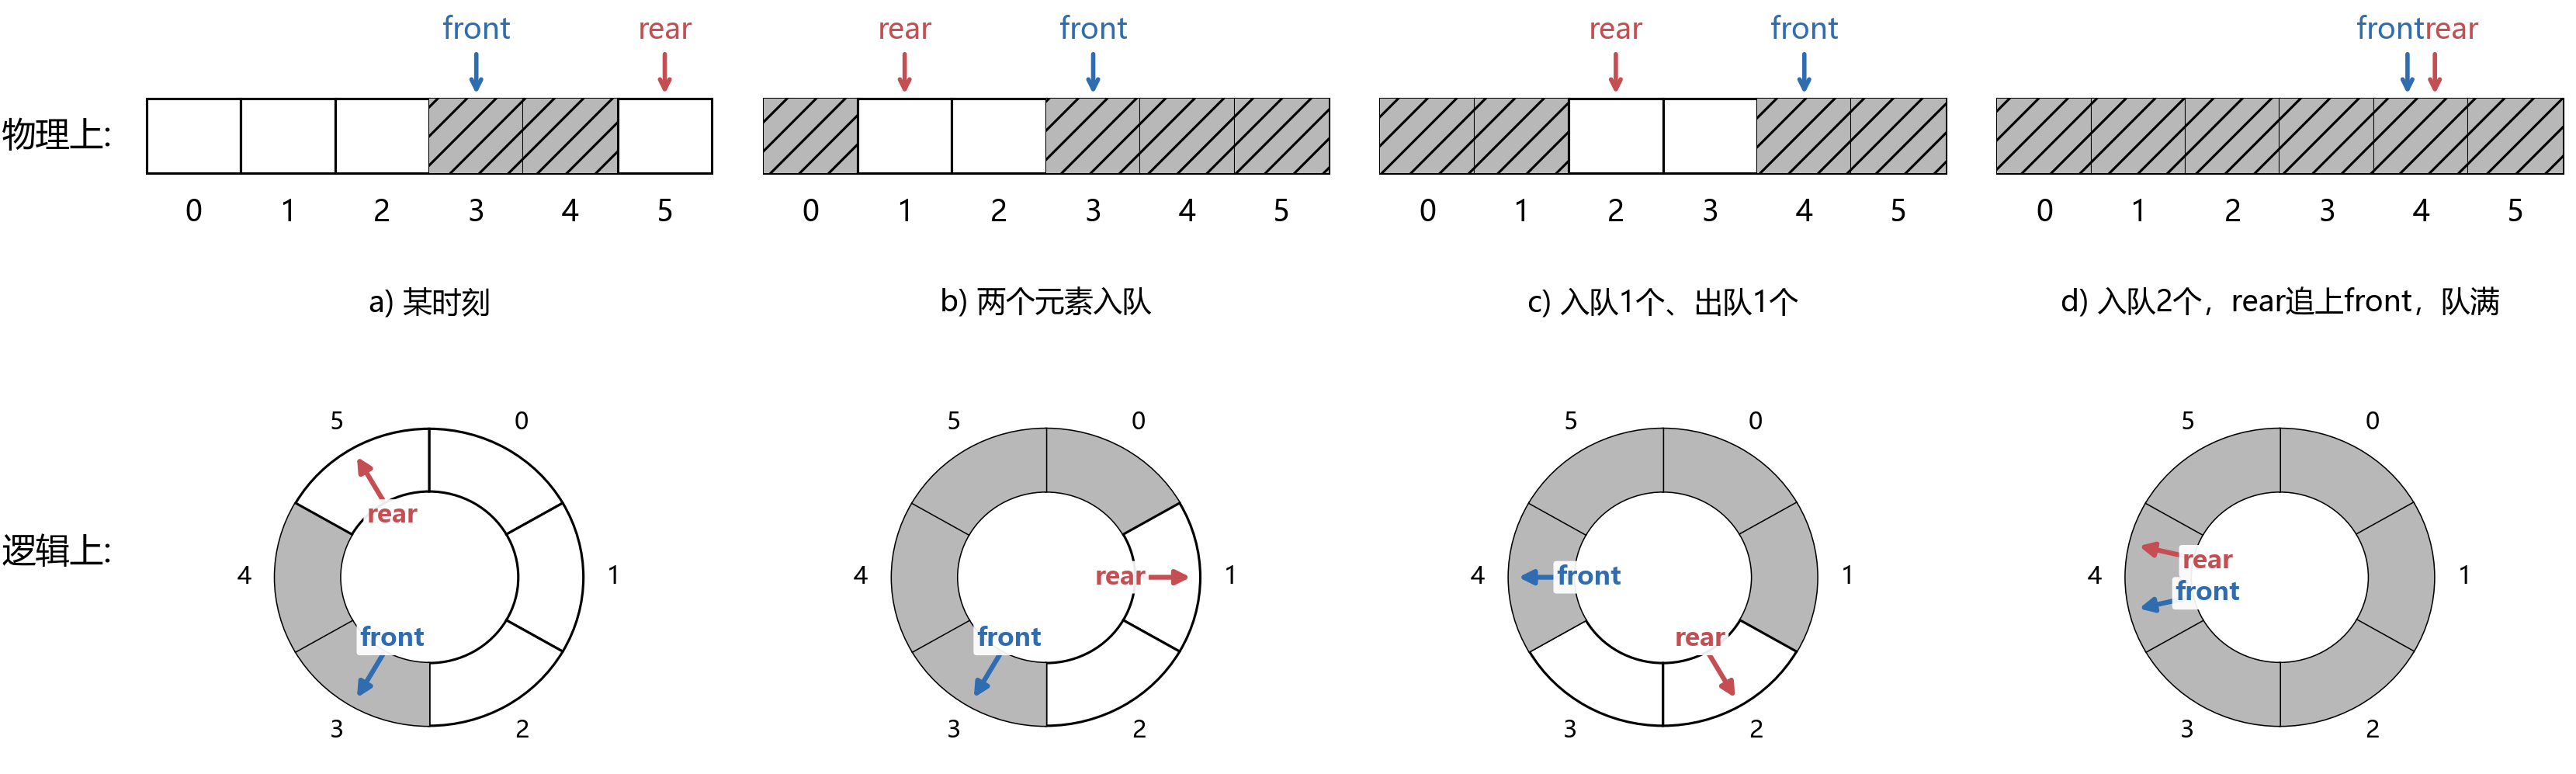
\includegraphics[width=1.10\textwidth]{assets/pics_and_ppts/ch3/循环队列示意图.png}
    \caption{循环队列示意图}
    \label{fig:循环队列示意图}
\end{figure}

这正是\term{循环队列}所要解决的问题。

循环队列不再把数组看成一条有起点、有终点的直线，而是把数组的首尾连接起来：当指针走到数组末尾时，就“绕回”数组开头，整个数组物理上是一条直线，但逻辑上是一个环，
因此叫\term{循环队列}或\term{环形队列}。

\textbf{因此，队列的顺序存储通常都会实现为循环队列}。

“回到起点”，代码上如何实现？举个例子某数组大小为100，下标为0-99，当rear的值已经为99时，如果不加以控制，下一步
将走到100，但我们希望它回到0。不难发现，这正是“取模”运算的功能。因此入队或出队时，若指针从99推移到100，我们将其对100取模，即可重新回到起点0：
\begin{cppcode}
    if(rear > MaxSize-1) {    // 若MaxSize为100，MaxSize-1为最大下标99
        rear = rear % MaxSize;
    }
\end{cppcode}

\begin{insightbox}
    在计算机科学中大家往往喜欢将“取模”和“取余”同等对待，但事实上存在负数参与运算时，取模（modulo）和取余（remainder）数学上的定义可能不同。“\%”运算符事实上更接近
    数学上的取余运算。但这里还是用“取模”来描述，原因在于二者在语感上有差异：“取余”关注的是除法“除完还剩多少”；而“取模”关注的是“映射到哪个模类/固定范围”。
    此处“\%”运算的语义更接近“取模”。
\end{insightbox}

还有第二个问题需要考虑。循环队列如何判断“队空”？可以简单地通过
\begin{bulk}
    \begin{center}
        front == rear \&\& front == 0
    \end{center}
\end{bulk}
来判断吗？经过分析发现是不可以的。因为队满的时候，上面的条件也可能成立。如图\ref{fig:循环队列示意图} ，对于d）所示场景，若再进行两次出队、两次入队，就可以
达成 front == rear \&\& front == 0 的条件，并且此时队列是满的。如何解决这个问题？相信大家自然地想到的做法是多维护一个字段，动态维护队列中当前元素个数：
\begin{cppcodeHighlight}[6]
    #define MaxSize 100
    struct SeqQueue {
        ElemType data[MaxSize];
        int front;
        int rear;
        int current_size;   // 新增字段
    };
\end{cppcodeHighlight}
这当然没问题。但更多教材给出的做法是少利用一个数组空间，通过 (Q.rear+1)\%MaxSize == Q.front 来作为队满的条件，如图\ref{fig:循环队列队满示意图}所示。
\begin{figure}[htbp]
    \centering
    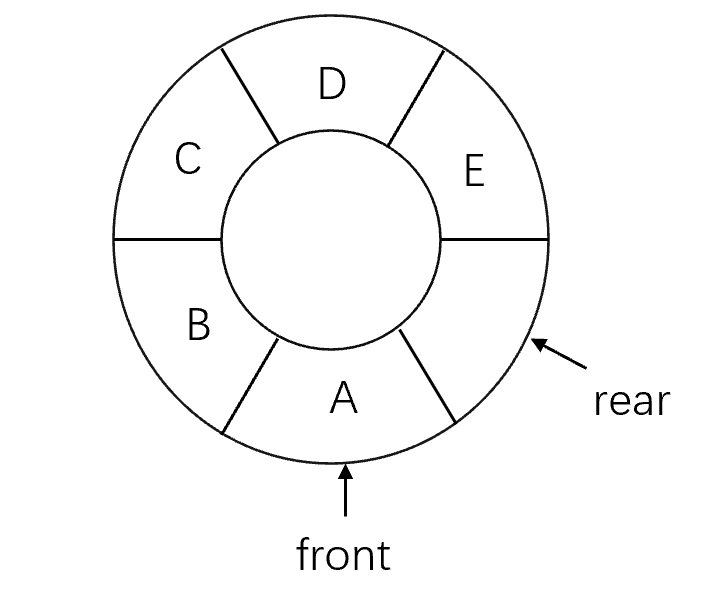
\includegraphics[width=0.28\textwidth]{assets/pics_and_ppts/ch3/循环队列队满示意图.png}
    \caption{队满示意图}
    \label{fig:循环队列队满示意图}
\end{figure}
我们这里遵从多数教材给出的做法，少利用一个数组空间，使用 (Q.rear+1)\%MaxSize == Q.front 来作为队满的条件。同时可以看到，在此做法下，除队空时front和rear初始化
为0之外，其余情况不可能出现 front == rear 的情况（因为我们少利用一个空间，所以rear永远无法追上front，最多只能在它后面一格）。所以可以将 front == rear 直接作为
判断队空的条件。

至此我们已经完成了所有“思维”上的准备，接下来给出循环队列的常见操作实现。

\minisection{1.初始化循环队列}
\begin{cppcode}
    int InitQueue(SeqQueue& q) {
        q.front = q.rear = 0;
        return 1;
    }
\end{cppcode}

\minisection{2.判断队空}
\begin{cppcode}
    int Empty(SeqQueue q) {
        if(q.front == q.rear) {
            return 1;
        }
        return 0;
    }
\end{cppcode}

\minisection{3.入队}
\begin{cppcode}
    int EnQueue(SeqQueue& q, ElemType e) {
        if( (q.rear+1) % MaxSize == q.front) {
            return 0;   // 队满，无法入队
        }

        // 先“放入元素”，再“推移指针”
        q.data[q.rear] = e;
        q.rear += 1;
        if(q.rear>=MaxSize) {
            q.rear = q.rear % MaxSize;
        }
        return 1;
    }
\end{cppcode}

\minisection{4.出队}
\begin{cppcode}
    int DeQueue(SeqQueue& q, ElemType& e) {
        if(Empty(q)) {
            return 0;   // 空队
        }

        // 先“取出元素”，再“推移指针”
        e = q.data[q.front];
        q.front += 1;
        if(q.front >= MaxSize) {
            q.front %= MaxSize;
        }
        return 1;
    }
\end{cppcode}

实际应用中，通常不会有“获取队列中的元素数量”的需求，这里笔者稍作提示：对于循环队列，可以通过下式在O(1)时间得到队列长度：
\begin{bulk}
    \begin{center}
        (rear-front+MaxSize) \% MaxSize
    \end{center}
\end{bulk}
而对于链队列，需要求队列长度，则需要遍历一遍队列（链表），时间复杂度为O(n)。\\

在解决实际问题时，有时会顺其自然地使用到两端均能入队、出队，或一端能入两端能出、两端能入一端能出的队列，它们通常被称为\term{双端队列}。{\color{red}\textbf{相关内容我们通过
习题2作为练习。}}

\section{栈的进一步理解}
提示：本节内容略有难度。\\


栈后进先出的特性，决定了其可以应用于一些很有趣的场景。我们这里先给出一般化的理解：许多场景下，可以用栈来保存这样的数据，即：\textbf{“那些仍然等待未来某个事件发生，并且
优先处理后来者”的数据。}现在看这句话过于抽象，不过别急，本节过后你的心会怦怦直跳。


\bookmark{bookmark:mark-3}{mark-3}
我们给出一例：现在假设天气预报已经报导了未来n天的温度，保存在一个数组temperatures[]中，请你设计一种算法，对于每一天i，找出其后方第一个温度高于第i天的日子。

最直接的办法就是“检查”每一天i，向后扫描，直到找到温度高于i的那一天，之后回到i+1，重复这个过程，伪代码如下所示：
\begin{cppcode}
    for(int i=0; i<n; i++) {
        int found = 0;
        for(int j=i+1; j<n; j++) {
            if(temperatures[j] > temperatures[i]) {
                // 找到了.
                found = 1;
                // j就是要找的那一天

                break;
            }
        }
        if(found == 0) {
            // 第i天的后面没有比第i天温度更高的了。
        }
    }
\end{cppcode}
显然这个算法时间复杂度为O(\(n^2\))。分析以上过程我们会发现，事实上我们做了很多查找是“不必要”的。比如，考虑temperatures[]输入如下：
\begin{bulk}
    \begin{center}
        25, 23, 19, 18, 20, 27, 26, 27
    \end{center}
\end{bulk}
当我们“检查”25时，就由前往后查找到了第一个27的位置，事实上此时我们就已经能够知道23的“答案天”就是27，并且19、18的“答案天”就是20。只不过，此时我们虽然已经
“看到了”这些信息，却没有把它们保存下来。于是，一个很自然的想法出现了：如果我们能通过某种手段将这些\textbf{尚未找到答案的天}记录下来，那么未来的温度出现
时，就可以立即检查这些等待中的天是否能够得到答案。当我们检查25时，将它记下来：
\begin{bulk}
    \begin{center}
        some\_structure: \{25\}
    \end{center}
\end{bulk}
检查23，some\_structure中没有元素会得到答案，将23记下来：
\begin{bulk}
    \begin{center}
        some\_structure: \{25, 23\}
    \end{center}
\end{bulk}
继续检查19、18：
\begin{bulk}
    \begin{center}
        some\_structure: \{25, 23, 19, 18\}
    \end{center}
\end{bulk}
当检查到20时，终于找到了19和18的答案，19和18两个元素期待的事情终于发生，因此将19和18从some\_structure中移出，将20记下来：
\begin{bulk}
    \begin{center}
        some\_structure: \{25, 23, 20\}
    \end{center}
\end{bulk}
你会惊奇地发现一件事情：留存在some\_structure中的温度序列一定是单调不增的，因为低温一定会在高温来到时“找到答案”而被移出。因此当新的温度t来到时，它能移出哪些
温度？其实只需要依次从some\_structure的尾部依次向前比较，“清除”掉some\_structure所有小于t的温度即可，这样一定不会漏。

说到这里你会发现，some\_structure正是满足“只会在一端进行插入删除”。或者换个角度想，当新温度t到来时，后进入some\_structure的元素一定要先被检查，因为后进入
的一定是更小的，如果都不能被t“清理掉”，前面的就更不会被清理掉。

这不就是栈吗！

想通了这一点，这个问题就变得非常简单：我们设一个栈s，保存所有“尚未找到答案”的天，并用一个数组ans[]保存已经得到的答案：ans[i]=j表示i的“答案天”是j。
如图\ref{fig:每日温度}，我们遍历一遍数组，依次检查temperatures[]中
的每一个温度temperatures[j] = t，将其与栈顶温度temperatures[s.top]进行比较，若t大于栈顶温度，则栈顶的这一天s.top的“答案天”就是j，并继续将t与新
的栈顶进行比较，重复这个过程，直至t不大于栈顶温度或栈空后，将当前检查的温度j入栈。检查完所有温度后，栈中剩余的这些天，就是后面没有温度高于他们的。
\begin{figure}[htbp]
    \centering
    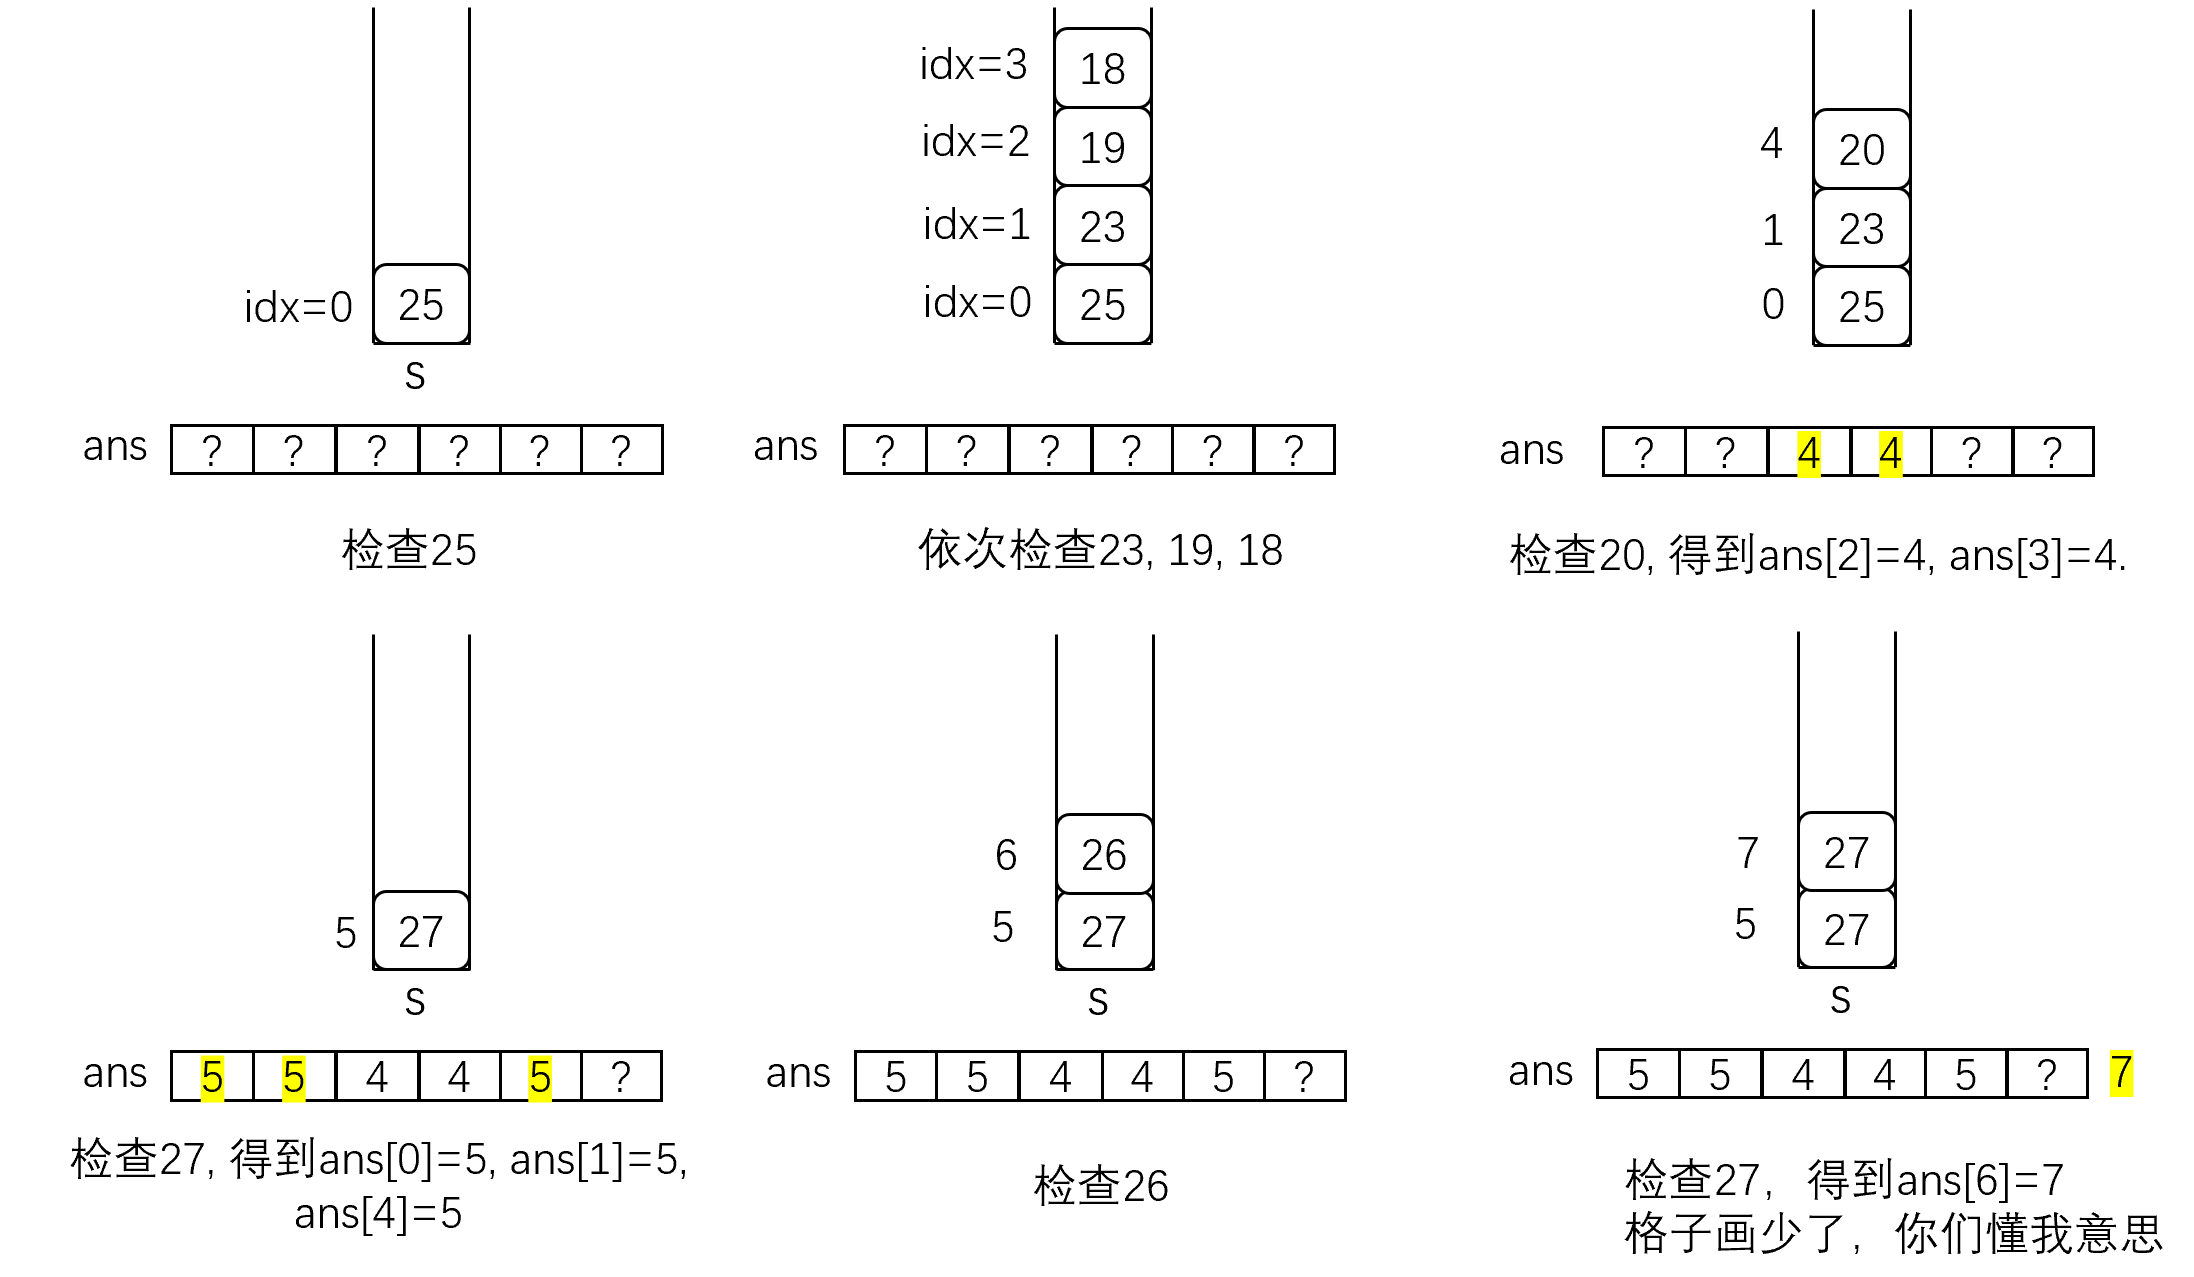
\includegraphics[width=0.81\textwidth]{assets/pics_and_ppts/ch3/每日温度.png}
    \caption{}
    \label{fig:每日温度}
\end{figure}
最后留在栈中的（下标为5和7的）两天，后面没有温度高于它们。伪代码如下所示：
\begin{cppcode}
    for(int i=0; i<n; i++) {
        while(!Empty(s) && temperatures[i]>temperatures[s.top]) {
            ans[s.top] = i;
            Pop(s);
        }
        Push(s, i);
    }
    while(!Empty(s)) {
        ans[s.top] = 0; // 这里拟用0表示后面不存在一天，比s.top这一天温度更高
        Pop(s);
    }
\end{cppcode}

该算法的时间复杂度为O(n)。至于为什么是O(n)，相比于上一种算法，该算法的提升在哪里，这里留给读者自行思考。可以看到，栈s中的元素是单调不增的，很多人喜欢
将这种元素具有单调性的栈称为\term{单调栈}，但笔者希望强调的更多是思考问题、解决问题的这个创造性的过程，次之才是：下次遇见类似的问题，可以用“单调栈”来解决。

相信通过该例大家已经建立了足够的感觉，我们来回看这句话：许多场景下，可以用栈来保存这样的数据，即：\textbf{“那些仍然等待未来某个事件发生，并且
优先处理后来者”的数据。}该例并非巧合，而是存在大量类似的问题，比如大名鼎鼎的\term{“表达式求值”}问题。

\subsection{表达式的转换与求值}
\label{sec:表达式的转换与求值}
表达式的转换与表达式的求值的过程中实际上也有类似上面的思想。
我们先来介绍中缀表达式、后缀表达式的概念。如果你已经了解二者的概念，并且能够熟练地将二者相互转换，请放心地直接跳至\bookmarkref{bookmark:mark-2}{mark-2}处。
我们平时书写算术表达式时，通常采用这样的形式：
\[
3+5
\]
如果表达式稍微复杂一些，例如：
\[
3+5\times2
\]
我们知道应该先计算乘法，再计算加法，这种运算符写在两个操作数之间的表达式，称为\textbf{中缀表达式（Infix Expression）}。

但是，计算机真的喜欢这样的表达式吗？

仔细观察上面的表达式：
\[
3+5\times2
\]
如果我们从左到右依次读取它，会先看到 $3+5$。
可是，此时却不能立即计算，因为后面的乘法具有更高的优先级。
也就是说，当我们看到一个运算符时，
有时可以立即计算，有时却必须\textbf{暂时把它保存起来}，
等待后面的运算符被处理之后才能决定。

如果再加入括号，情况会变得更加复杂：
\[
(3+5)\times2
\]
这时我们不仅需要考虑运算符的优先级，
还需要处理括号所带来的运算顺序。\\

如果我们将
\[
(3+5)\times2
\]
改写成
\[
3\;5\;2\;\times \;+
\]
此时我们再从左向右读取它，你会发现：
\begin{enumerate}
    \item 读取 $3$；
    \item 读取 $5$；
    \item 读取 $2$；
    \item 读取 $\times$，将 $5$ 和 $2$ 相乘，得到10，表达式变成了3 10 +；
    \item 读取 $+$，将 $3$ 和 $10$ 相加，得到最终结果。
\end{enumerate}

整个计算过程不需要我们再判断“乘法是不是应该优先计算”，
因为\textbf{运算符出现的位置本身，就已经把运算顺序表达出来了}。

这种将运算符写在其操作数之后的表达式，称为\textbf{后缀表达式（Postfix Expression）}，也称为\textbf{逆波兰表达式（Reverse Polish Notation，RPN）}。
我们再给出几例。
中缀表达式
\[
b\times c+(a-d)
\]
的后缀形式为：
\[
bc\times ad-+
\]
至于如何手动将中缀转后缀，限于篇幅，此处不再给出，请大家参考CoreLoop本人相关DLC。

中缀表达式
\[
a+b\times c-(b-d)\div e
\]
的后缀形式为：
\[
abc\times +bd-e\div -
\]

在后缀表达式中，每一个运算符都紧跟在它所需要的操作数之后，
因此不需要再使用括号，也不需要额外规定运算符的优先级。

\bookmark{bookmark:mark-2}{mark-2}
\minisection{栈与表达式求值}
我们首先考虑较简单的，计算机如何求值后缀表达式。

计算机按照从左到右的顺序处理后缀表达式，当看到一个数字时，应该把它放在哪里？当看到一个运算符时，又应该从哪里取出它所需要的操作数？

例如，对于：
\[
3\;5\;2\;\times\;+
\]
当读取到 $\times$ 时，需要取出最近读取的两个操作数 $5$ 和 $2$；

而计算出 $5\times2=10$ 后，
又需要把结果暂时保存起来，
等待后面的 $+$。

这种“\textbf{最后保存的操作数最先被取出使用}”的特点，恰好符合栈的\textbf{后进先出}原则。于是，后缀表达式求值的算法就变得很好理解：
对于后缀表达式，我们从左到右依次读取每一个元素：
\begin{itemize}
    \item 如果读取到的是操作数，则将其压入栈中；
    \item 如果读取到的是运算符，则从栈中弹出所需数量的操作数，
          完成运算后，再将运算结果压入栈中。
\end{itemize}
当整个表达式处理完毕后，栈中剩下的唯一元素就是整个表达式的计算结果。

后缀表达式最重要的特点并不是“把运算符放到了后面”，而是：
\begin{quote}
\textbf{它把原本隐藏在括号和运算符优先级中的运算顺序，
直接编码到了表达式的排列顺序中。}
\end{quote}
因此，对于后缀表达式，计算机不再需要理解“谁的优先级更高”，也不需要处理括号的嵌套关系，只需要从左到右读取表达式，并按照遇到的运算符立即进行计算即可。求
后缀表达式
\[
abc\times +bd-e\div -
\]
的值的过程如表\ref{tab:后缀表达式求值过程}所示。

\begin{table}[h]
    \centering
    \caption{后缀表达式求值过程}
    \label{tab:后缀表达式求值过程}

    \renewcommand{\arraystretch}{1.4}

    \begin{tabularx}{\textwidth}{
        >{\centering\arraybackslash}p{0.07\textwidth}
        >{\centering\arraybackslash}p{0.09\textwidth}
        >{\centering\arraybackslash}p{0.12\textwidth}
        >{\raggedright\arraybackslash}X
        >{\centering\arraybackslash}p{0.25\textwidth}
    }

        \toprule
        步骤
        & 扫描项
        & 项类型
        & 动作
        & 栈中内容（栈底 $\rightarrow$ 栈顶）
        \\
        \midrule

        1
        & $a$
        & 操作数
        & $a$ 入栈
        & $a$
        \\

        2
        & $b$
        & 操作数
        & $b$ 入栈
        & $a,\ b$
        \\

        3
        & $c$
        & 操作数
        & $c$ 入栈
        & $a,\ b,\ c$
        \\

        4
        & $\times$
        & 运算符
        & 弹出 $b$、$c$，计算 $b\times c$，
          将结果 $bc$ 入栈
        & $a,\ bc$
        \\

        5
        & $+$
        & 运算符
        & 弹出 $a$、$bc$，计算 $a+bc$，
          将结果入栈
        & $a+bc$
        \\

        6
        & $b$
        & 操作数
        & $b$ 入栈
        & $a+bc,\ b$
        \\

        7
        & $d$
        & 操作数
        & $d$ 入栈
        & $a+bc,\ b,\ d$
        \\

        8
        & $-$
        & 运算符
        & 弹出 $b$、$d$，计算 $b-d$，
          将结果入栈
        & $a+bc,\ b-d$
        \\

        9
        & $e$
        & 操作数
        & $e$ 入栈
        & $a+bc,\ b-d,\ e$
        \\

        10
        & $\div$
        & 运算符
        & 弹出 $b-d$、$e$，计算
          $\dfrac{b-d}{e}$，将结果入栈
        & $\displaystyle a+bc,\ \frac{b-d}{e}$
        \\

        11
        & $-$
        & 运算符
        & 弹出 $a+bc$、$\dfrac{b-d}{e}$，
          计算 $\displaystyle a+bc-\frac{b-d}{e}$，
          将结果入栈
        & $\displaystyle a+bc-\frac{b-d}{e}$
        \\

        \bottomrule

    \end{tabularx}
\end{table}


事实上，计算机可以\textbf{直接求值中缀表达式}，而无需先将中缀表达式转换为后缀表达式，再进行求值。接下来我们来看计算机如何直接求值中缀表达式。
与后缀表达式不同的是，当计算机从左到右读取中缀表达式时，遇到一个运算符op后，不能总是立即计算。某些运算符必须暂时保存下来，等待后面的运算符出现之后，
才能决定自己什么时候参与计算。有了前面的思想很容易知道，扫描过程中遇到的运算符op就是\textbf{“那些仍然等待未来某个事件发生，并且优先处理后来者”}的数据。

于是，一个非常自然的设计出现了：

\begin{itemize}
    \item \textbf{操作数栈：}保存当前暂时不能参与运算的操作数以及中间计算结果；
    \item \textbf{运算符栈：}保存当前暂时不能执行的运算符。
\end{itemize}

当计算机从左到右读取一个中缀表达式时，可以按照下面的规则进行处理：

\begin{enumerate}
    \item 从左到右依次读取中缀表达式中的每一个元素。
    \item 如果读取到的是操作数，则将其压入操作数栈。
    \item 如果读取到的是左括号，则将其压入运算符栈。
    \item 如果读取到的是右括号，则不断弹出运算符栈的栈顶运算符，
    从操作数栈中取出相应的操作数进行计算，并将计算结果重新压入操作数栈，
    直到遇到左括号为止。最后将左括号弹出并丢弃。
    \item 如果读取到的是运算符，则比较当前运算符与运算符栈栈顶运算符的优先级：
    \begin{itemize}
        \item 如果运算符栈为空，或者栈顶为左括号，或者当前运算符的优先级高于栈顶运算符，
        则将当前运算符压入运算符栈；
        \item 否则，不断弹出栈顶运算符，从操作数栈中取出相应的操作数进行计算，
        并将计算结果重新压入操作数栈，直到当前运算符可以入栈为止，
        然后将当前运算符压入运算符栈。
    \end{itemize}
    \item 中缀表达式读取完毕后，不断弹出运算符栈中的运算符，
    从操作数栈中取出相应的操作数进行计算，并将计算结果重新压入操作数栈。
    \item 当运算符栈为空时，操作数栈中剩余的唯一元素即为整个中缀表达式的计算结果。
\end{enumerate}

这样，我们就不需要先将中缀表达式转换成后缀表达式，而是可以直接在读取中缀表达式的过程中完成计算。

这个过程我没有画图，并不是因为懒，而是相信通过前面的寻找温度的例子，你已经对类似场景建立了足够的直觉。如果你还没有搞清楚“栈与表达式”是怎么回事，
可以参考CoreLoop本书相关的DLC。


\minisection{*栈与表达式转换}
根据前面的介绍，事实上计算机可以借助两个栈，直接计算中缀表达式的值。但出于某种原因，这里我们依然介绍一下计算机如何借助栈将中缀表达式转换为后缀表达式。
有了前面的内容相信大家已经能够自行想出正确的做法了。我们这里直接给出：
\begin{enumerate}
    \item 从左到右依次读取中缀表达式中的每一个元素。
    \item 如果读取到的是操作数，则直接将其加入后缀表达式。
    \item 如果读取到的是左括号，则将其压入运算符栈。
    \item 如果读取到的是右括号，则不断弹出运算符栈的栈顶元素，
    并将其加入后缀表达式，直到遇到左括号为止。
    左括号弹出后丢弃，不加入后缀表达式。
    \item 如果读取到的是运算符，则比较它与运算符栈栈顶运算符的优先级：
    \begin{itemize}
        \item 如果栈为空，或者栈顶为左括号，或者当前运算符的优先级高于栈顶运算符，
        则将当前运算符压入栈中；
        \item 否则，不断弹出栈顶运算符并加入后缀表达式，
        直到当前运算符可以入栈为止。
    \end{itemize}
    \item 中缀表达式读取完毕后，将运算符栈中剩余的运算符依次弹出，
    并加入后缀表达式。
\end{enumerate}
整个过程的核心其实非常简单：
\begin{quote}
\textbf{操作数直接输出，运算符暂存于栈中；当一个运算符已经可以确定其位置时，
就将它从栈中弹出并输出。}
\end{quote}
中缀表达式
\[
a+b\times c-(b-d)\div e
\]
转后缀表达式的过程如表\ref{tab:中缀转后缀过程}所示。
\begin{table}[htbp]
    \centering
    \caption{中缀表达式转换为后缀表达式的过程}
    \label{tab:中缀转后缀过程}

    \renewcommand{\arraystretch}{1.35}

    \begin{tabularx}{\textwidth}{
        >{\centering\arraybackslash}p{0.06\textwidth}
        >{\centering\arraybackslash}p{0.09\textwidth}
        >{\centering\arraybackslash}p{0.12\textwidth}
        >{\raggedright\arraybackslash}X
        >{\centering\arraybackslash}p{0.20\textwidth}
        >{\centering\arraybackslash}p{0.20\textwidth}
    }

        \toprule
        步骤
        & 扫描项
        & 项类型
        & 动作
        & 运算符栈（栈底 $\rightarrow$ 栈顶）
        & 后缀表达式
        \\
        \midrule

        1
        & $a$
        & 操作数
        & $a$ 直接输出
        &
        &
        $a$
        \\

        2
        & $+$
        & 运算符
        & 栈为空，$+$ 入栈
        &
        $+$
        &
        $a$
        \\

        3
        & $b$
        & 操作数
        & $b$ 直接输出
        &
        $+$
        &
        $ab$
        \\

        4
        & $\times$
        & 运算符
        & $\times$ 的优先级高于栈顶的 $+$，
          $\times$ 入栈
        &
        $+,\ \times$
        &
        $ab$
        \\

        5
        & $c$
        & 操作数
        & $c$ 直接输出
        &
        $+,\ \times$
        &
        $abc$
        \\

        6
        & $-$
        & 运算符
        & $-$ 的优先级低于栈顶的 $\times$，
          弹出 $\times$ 并输出；
          $-$ 的优先级与栈顶的 $+$ 相同，
          弹出 $+$ 并输出；然后 $-$ 入栈
        &
        $-$
        &
        $abc\times+$
        \\

        7
        & $($
        & 左括号
        & 左括号直接入栈
        &
        $-,\ ($
        &
        $abc\times+$
        \\

        8
        & $b$
        & 操作数
        & $b$ 直接输出
        &
        $-,\ ($
        &
        $abc\times+b$
        \\

        9
        & $-$
        & 运算符
        & 栈顶为左括号，不进行优先级比较，
          $-$ 直接入栈
        &
        $-,\ (,\ -$
        &
        $abc\times+b$
        \\

        10
        & $d$
        & 操作数
        & $d$ 直接输出
        &
        $-,\ (,\ -$
        &
        $abc\times+bd$
        \\

        11
        & $)$
        & 右括号
        & 依次弹出栈顶运算符并输出；
          遇到左括号后将其弹出，但不输出
        &
        $-$
        &
        $abc\times+bd-$
        \\

        12
        & $\div$
        & 运算符
        & $\div$ 的优先级高于栈顶的 $-$，
          $\div$ 入栈
        &
        $-,\ \div$
        &
        $abc\times+bd-$
        \\

        13
        & $e$
        & 操作数
        & $e$ 直接输出
        &
        $-,\ \div$
        &
        $abc\times+bd-e$
        \\

        14
        & 结束
        & —
        & 扫描结束，将栈中剩余的运算符依次弹出并输出
        &
        —
        &
        $abc\times+bd-e\div-$
        \\

        \bottomrule

    \end{tabularx}
\end{table}


\clearpage%%%%%%%%%%%%%%%%%%%%%%%%%%%%%%%%%%%%%%%%%%%%%%%%%%%%%%%%%%%%%%%%%%%%%%%%%%%%%%%%%%%%%%%%%%%%%%%%%%%%%%%%%%%%%%%%%%%%%%%%%%%%%%%%%%%%%%%%%%
\begin{exercise}
    1. [多选]下列说法正确的是$\underline{\hspace{1cm}}$。\\
A. 栈是一种有特殊要求的线性表。\\
B. 队列是一种有特殊要求的线性表。\\
C. 最先入栈的元素一定最先出栈。\\
D. 最先入队的元素一定最先出队。\\

    2. 以下哪一项不是栈可以进行的操作？$\underline{\hspace{1cm}}$\\
A. 将元素压入栈中\\
B. 判断栈是否为空\\
C. 删除栈底元素\\
D. 将栈置为空栈\\

    3. 以下哪一项不是队列可以进行的操作？$\underline{\hspace{1cm}}$\\
A. 将元素插入队尾\\
B. 获取队首元素的值\\
C. 获取位序为i的元素的值\\
D. 位序为i的元素出队\\

    4. 某个栈，元素的入栈序列是 $$ 1,2,3,4 $$ 则以下序列中，不可能作为出栈序列的是：$\underline{\hspace{1cm}}$\\
A. 2, 1, 3, 4\\
B. 2, 3, 4, 1\\
C. 3, 2, 4, 1\\
D. 3, 4, 1, 2\\

    5. 关于时间复杂度，以下说法正确的是：\\
A. 顺序栈的 Push 和 Pop 时间均为 \(O(n)\)\\
B. 链栈的 Push 和 Pop 均可实现为 \(O(1)\)\\
C. 使用单链表实现队列时，只要有 head 指针，入队和出队均可实现为 \(O(1)\)\\
D. 循环队列的入队操作必须移动大量元素，因此时间复杂度为 O(n)\\

    6. 采用数组实现容量为 \(N\) 的循环队列，并规定：\\
front 指向队首元素；\\
rear 指向下一个插入位置；\\
front和rear初始全部指向下标\(N-1\)处，队列采用保留一个空闲位置的方式区分队满和队空。

则判断队列为空和队满的条件分别为：\\
A. front == 0 \&\& rear == 0, rear + 1 == front\\
B. front == 0 \&\& rear == 0, (rear + 1) \% N == front\\
C. front == rear, rear + 1 == front\\
D. front == rear, (rear + 1) \% N == front \\

    7. [多选]某同学做了如下设计：采用一个长度为100的数组实现两个栈S1和S2。该同学规定两栈栈底分别在两个端点处，栈顶向中间生长，如图\ref{fig:共享栈}。
    同时规定两栈栈顶元素相邻时，存储空间满，均无法再入栈。
\begin{figure}[htbp]
    \centering
    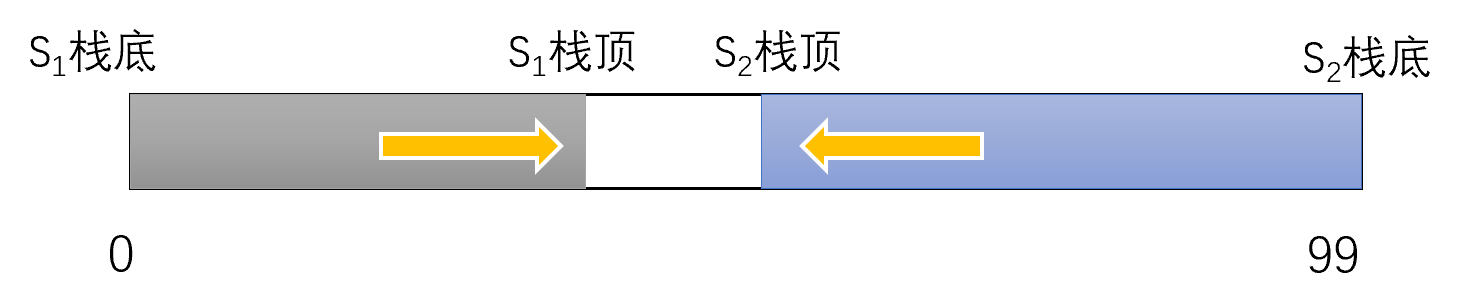
\includegraphics[width=0.67\textwidth]{assets/pics_and_ppts/ch3/共享栈.png}
    \caption{}
    \label{fig:共享栈}
\end{figure}
    以下说法中正确的是$\underline{\hspace{1cm}}$\\\\
\textbf{A.} 两栈入栈时间复杂度均为O(1)\\
\textbf{B.} 设两栈元素数量分别为n、m，则两栈栈顶元素的出栈时间复杂度分别为O(n)、O(m)\\
\textbf{C.} 要计算两栈栈中已有元素数量之和，时间复杂度为O(1)\\\\
\textbf{D.} 若S1.top初始化为-1，S2.top初始化为100，且两个栈顶指针始终指向各自的栈顶元素，则S1.top+1==S2.top时，空间满，两栈均无法再入栈\\
\textbf{E.} 若S1.top初始化为-1，S2.top初始化为100，且两个栈顶指针始终指向各自的栈顶元素，则可能出现S1.top>S2.top\\
\textbf{F.} 若S1.top初始化为0，S2.top初始化为99，且两个栈顶指针始终指向各自栈顶元素的下一个位置，则S1.top+1==S2.top时，空间满，两栈均无法再入栈\\
\textbf{G.} 若S1.top初始化为0，S2.top初始化为99，且两个栈顶指针始终指向各自栈顶元素的下一个位置，则可能出现S1.top>S2.top\\


    8. 一个初始为空的栈和一个初始为空的队列，都依次接收：
$$ 1,2,3,4,5 $$
如果只允许进行正常的入栈、出栈、入队、出队操作，关于它们能够产生的输出顺序，下列说法正确的是：\\
A. 栈和队列都可以产生任意排列\\
B. 栈只能产生一种输出顺序，队列也只能产生一种输出顺序\\
C. 队列的输出顺序固定为 \(1,2,3,4,5\)，而栈的输出顺序受到栈操作过程限制\\
D. 栈的输出顺序固定为 \(5,4,3,2,1\)，队列的输出顺序受到操作过程限制\\
    
    9.[多选]假设输入序列是1,2,3,4,5，利用两个队列进行出入队操作，不可能的输出序列有$\underline{\hspace{1cm}}$\\
A. 5,4,3,2,1\\
B. 5,1,2,3,4\\
C. 5,2,3,1,4\\
D. 2,3,4,5,1\\

    10. [多选]与循环队列相比，链式队列$\underline{\hspace{1cm}}$\\
A. 优点是进队和出队时间复杂度更低\\
B. 优点是长度可以在内存限制内动态变化\\
C. 缺点是节点除数据外需要额外的存储空间存放指针\\
D. 缺点是不能根据队首和队尾指针以O(1)时间算出队列长度\\

    11. 假设某队列采用带头结点的循环双链表实现，第一个数据节点表示队头，最后一个数据节点表示队尾。若只设头指针指向头节点，则进队和出队的时间复杂度分别为：\\
A. O(1), O(1) \\
B. O(1), O(n)\\
C. O(n), O(1)\\
D. O(n), O(n)\\

    12. （某年408真题）现有队列Q和栈S，初始时Q中的元素依次是1,2,3,4,5,6（1在队头），S为空。若仅允许下列的3种操作：\Circled{1}出队并输出出队元素；\Circled{2}出队
    并将出队元素入栈；\Circled{3}出栈并输出出栈元素。则不能得到的输出序列是$\underline{\hspace{1cm}}$\\
A. 1,2,5,6,4,3\\
B. 2,3,4,5,6,1\\
C. 3,4,5,6,1,2\\
D. 6,5,4,3,2,1\\

    13. （某年408真题）某队列允许在其两端进行入队操作，但仅允许在一端进行出队操作。若元素a,b,c,d,e依次入此队列后再进行出队操作，则不可能得到的出队序列是$\underline{\hspace{1cm}}$\\
A. b,a,c,d,e\\
B. d,b,a,c,e\\
C. d,b,c,a,e\\
D. e,c,b,a,d\\

    14. （某年408真题）初始为空的队列Q的一端仅能进行入队操作，另外一端既能进行入队操作，又能进行出队操作。若Q的入队序列是1,2,3,4,5，则不能得到的出队序列是$\underline{\hspace{1cm}}$\\
A. 5,4,3,1,2\\
B. 5,3,1,2,4\\
C. 4,2,1,3,5\\
D. 4,1,3,2,5\\

    15. （某年408真题）假设栈初始为空，将中缀表达式a/b+(c*d-e*f)/g转换为等价的后缀表达式的过程中，当扫描到f时，栈中的元素依次是$\underline{\hspace{1cm}}$\\
A. +(*-\\
B. +(-*\\
C. /+(*-*\\
D. /+-*\\

    16. （某年408真题）若栈S1中保存整数，栈S2中保存运算符，函数F()依次执行下述的各步操作：\\
    1) 从S1中依次弹出两个操作数a和b；\\
    2) 从S2中弹出一个运算符op；\\
    3) 执行相应的运算b op a；\\
    4) 将运算结果压入S1中。\\
    假定S1中的操作数依次是5,8,3,2（2在栈顶），S2中的运算符依次是*, -, +（+在栈顶）。调用3次F()后，S1栈顶保存的值是$\underline{\hspace{1cm}}$\\
    A. -15\\
    B. 15\\
    C. -20\\
    D. 20\\

    *17. 某游戏服务器持续记录某位名为CoreLoop的玩家的网络延迟情况。现假设服务器连续记录了 \(n\) 个时刻的网络延迟，第 \(i\) 个时刻的延迟为 delay[i]，
    这些数值均为正整数。为防止数值闪动，该服务器将时刻i的近k个时刻延迟的最大值作为该玩家在时刻i的\textbf{显示延迟}。
    也就是说，时刻i的显示延迟为：
    \[
        max(delay[max(0, i-k+1)], delay[max(0, i-k+2)], ..., delay[i])
    \]

    如，对于：
    \[
        delay[] = {40, 33, 38, 37, 42, 35}
    \]

    k=3时，显示延迟为
    \[
        ans[]   = {40, 40, 40, 38, 42, 42}
    \]

    k=4时，显示延迟为
    \[
        ans[]   = {40, 40, 40, 40, 42, 42}
    \]
    请你设计一个尽可能高效的算法，求出该玩家这n个时刻的\textbf{显示延迟}。
    \begin{cppcode}
    // 将时刻0到n-1的显示延迟保存在ans[]数组下标0到n-1处。
        void MaxDelay(int delay[], int n, int k, int ans[]) {

        }
    \end{cppcode}



\end{exercise}
\clearpage

\begin{exerciseanswer}
    1. 选ABD。\\

    2. 选C。栈的插入删除只能在栈顶进行，C错误。\\

    3. 选D。对于C项，队列仅要求队首元素可以出队，但没要求仅队首元素可以被读取。你当然可以为队列实现获取第i个元素的函数接口，但通常来说我们使用队列的场景往往不会有这个需求。
    额外提示：你当然可以为你的“队列”实现第i个元素“出队”的函数接口，但这样做的话，你所实现的数据结构就不能叫做\term{队列}了。\\

    4. 选D。2134可由入入出出入出入出达成；2341可由入入出入出入出出达成；3241可由入入入出出入出出达成；栈满足后进先出，如论如何4一定比3先出，2一定比1先出，D无法达成。\\

    5. 选B。对于A，顺序栈的Push和Pop操作均在顺序表的表尾实现，时间均可达到O(1)；对于C，仅有head指针的单链表实现“头删”，即出队，可达到O(1)，但要实现“尾删”，即出队，
    则需要先找到最后一个节点，时间为O(n)。单链表中额外记录一个尾指针rear，则入队和出队均可达成O(1)时间。对于D，循环队列的入队和出队无需移动元素。\\

    6. 选D。通过本题给了我们一个提示，对于循环队列来说，初始front和rear不一定非要指向0，因为从环的几何结构来讲，“队首元素”保存在0位置和保存在i位置是没有区别的。
    仅有初始状态（队空）会满足front == rear。\\

    7. 选A、C、D、G。对于B，无论栈中有多少个元素，一次出栈操作只需要访问当前栈顶元素，然后修改栈顶指针即可，时间复杂度为O(1)。\\
    对于C，可由两栈的栈顶下标直接分别计算得到两栈的元素数量，时间均为O(1)，再相加即可得到总数量，总体时间为O(1)，C正确；\\
    对于D，要注意：当栈S2中没有元素，而栈S1将空间全部占满时，同样可以用S1.top+1==S2.top判断空间满，当S2将空间占满时同样如此，D正确；\\
    E、F显然错误；\\
    对于G，当栈满时，S1.top指向S1栈顶元素的下一个位置，即S2的栈顶元素位置；对应地，S2.top指向S1的栈顶元素位置，S1.top>S2.top成立，G正确。\\

    8. 选C。队列的特性决定了第i个入队的元素一定是第i个出队的，而栈则不同，栈的出栈顺序是会受到操作过程影响的，{\color{red}\textbf{参考本习题第4题}}。\\

    9. 选AC。\\

    10. 选BCD。\\

    11. 选A。对于循环双链表，可以在O(1)时间立即拿到尾节点指针，因此在头、尾操作均为O(1)。\\

    12. 选C。A项可以通过\Circled{1}\Circled{1}\Circled{2}\Circled{2}\Circled{1}\Circled{1}\Circled{3}\Circled{3}得到；
    B项可通过\Circled{2}\Circled{1}\Circled{1}\Circled{1}\Circled{1}\Circled{1}\Circled{3}得到；
    D项输入与输出刚好相反，显然通过栈就能逆序：\Circled{2}\Circled{2}\Circled{2}\Circled{2}\Circled{2}\Circled{2}\Circled{3}\Circled{3}\Circled{3}\Circled{3}\Circled{3}\Circled{3}。
    对于C，3在1、2前输出，因此1、2必按顺序先入栈，所以1必晚于2输出，C错误。\\

    13. 选C。这是一个非常有意思的题。不妨假设仅有左边能出队。无论如何a一定先入队，摆在最中央的位置。接下来，每一个元素入队，你都可以选择将其“摆在队中已有元素的左边或右边”。所以你需要
    以a为中心努力地去构造四个选项所给出的序列。如A选项要求的序列是b,a,c,d,e，于是你将b摆在a左边，将c摆在ba的右边，将d摆在bac的右边，再将e摆在bacd的右边，便得到
    了A项所要求的序列，从左边出队，便得到了b,a,c,d,e。B、D项也都可以通过同样的方法得到。\\

    14. 选D。\\
    
    15. 选B。详细过程已经在\ref{sec:表达式的转换与求值}中介绍过，不再赘述。\\

    16. 选B。本题比较简单，注意出栈顺序别搞错，同时注意二元运算符op的操作数顺序是b op a而不是a op b，不要搞错就行。\\

    17. 这个问题如果你在思考的过程中自然地想到了使用某种“一端进，两端出”的数据结构，那么你可以开一瓶香槟庆祝一下。如果你只想到了时间复杂度为\(O(n\times k)\)的算法，
    你应该惩罚自己周末不许出去玩。

    本题最容易想到的方法是：从前向后遍历一遍delay[]数组，检查每一个延迟数值delay[i]时，从i向前找，直到遇见下标0或i-k+1的元素，在这个过程中记录下一个最大值，作为
    i时刻的延迟最大值，即ans[i]。该方法的时间复杂度为\(O(n\times k)\)。当k较大时，复杂度可能接近\(O(n^2)\)。\\

    但是，以上方法与“天气预报问题”（见\bookmarkref{bookmark:mark-3}{mark-3}处）的朴素解法有着类似的问题：当我们检查后面的元素时，前面的元素其实已经被检查过若干
    遍了。我们能不能在每个元素第一次被检查的时候，就想办法将它保存到某个结构some\_structure中，直至该元素“不可能成为后面任何一个i的解”，再将它丢弃呢？\\

    我们从前向后遍历，当检查下标为i的元素时：\\
    1）显然，下标<=i-k的元素已经不再可能成为后面任何一个元素（包括i）的解。所以需要将所有下标<=i-k的元素移出some\_structure。这正是“先进先出”。\\
    2）当我们检查i时，由于i可以作为自己的解，所以some\_structure中所有值小于i的元素均已不再可能成为后面任何一个元素的解，移出它们。经过分析不难发现，
    该特性决定了some\_structure中元素单调不增。所以移出时应该将delay[i]与“后进来的”元素先比较。

    所以这个结构应该是一个“尾端能进能出、首端能出”的一个结构。并且当检查元素i时，移出满足上述1）、2）条件的元素后，队首元素就是该元素i的解。
    
    如正文中介绍过，通常称其为\term{双端队列}。此处我们是在解决问题（而不是封装某种数据结构给别人或自己复用），因此
    我们不兴师动众地封装一个“双端队列”的数据结构，并为他写出“首端出队”、“尾端入队、尾端出队”等操作，而是直接将操作展开，作为逻辑的一部分实现。完整代码如下所示。
    \begin{cppcode}
        void MaxDelay(int delay[], int n, int k, int ans[]) {
            // deque[] 保存候选元素的下标。
            // deque[front] 是队首，deque[rear - 1] 是队尾。
            int deque[n];
            int front = 0;
            int rear = 0;

            for (int i = 0; i < n; i++) {
                while (front < rear && deque[front] <= i - k) {
                    // 动态维护队首元素（i的解）
                    front++;     // 注意入队元素一定不会超过n，因此不用考虑循环
                }

                // 移除所有不可能再成为最大值的元素。
                while (front < rear &&
                    delay[deque[rear - 1]] <= delay[i]) {
                    rear--;
                }

                // 当前元素加入队尾。
                deque[rear] = i;
                rear++;

                // 队首就是当前窗口中的最大值。
                ans[i] = delay[deque[front]];
            }
        }
    \end{cppcode}
    

\end{exerciseanswer}